%Use 16:9
\documentclass[dvipsnames]{beamer}
\title{Reverse Mode Automatic Differentiation: Unraveling Expression Graphs \& Library Magic}
\author{Steve Bronder}
\date{September 2025}
\setbeameroption{show notes}
\setbeamertemplate{note page}{\pagecolor{yellow!5}\insertnote}\usepackage{palatino}
%\setbeameroption{show notes on second screen=right} % Both

\usepackage{graphicx} % Required for inserting images
\usepackage{xcolor}
\usepackage{comment}
\definecolor{codebg}{HTML}{1f2937} % GitHub Dark background
\usepackage[newfloat]{minted}
\usepackage{fontspec}
\setmonofont{Fira Code}
\usepackage{enumitem}
\setlist[itemize,1]{label=-}
% Colors
\usepackage{xcolor}

% Use the same style everywhere
\usemintedstyle{monokai}

% Global minted defaults (including background)
\setminted{
  breaklines,
  breakanywhere,
%  linenos,
  numbersep=6pt,
  fontsize=\footnotesize,
  xleftmargin=1em,
  tabsize=2,
  bgcolor=codebg,             % <<< make minted's background dark
}

% C++-specific tweaks
\setminted[c++]{
  mathescape,
  escapeinside=||,
}


% Make line numbers readable on dark bg (optional but nice)
\makeatletter
\renewcommand\theFancyVerbLine{%
  \textcolor{white!60}{\arabic{FancyVerbLine}}%
}
\makeatother

% tcolorbox wrapper: use the same background + a subtle frame
\usepackage[most]{tcolorbox}
\tcbuselibrary{minted,skins,breakable}
\newtcblisting{cppcode}[1][]{
  listing engine=minted,
  minted language=c++,
  minted style=monokai,  % keep in sync
  minted options={
    linenos,autogobble,breaklines,fontsize=\footnotesize,
    mathescape,escapeinside=||,
 %   bgcolor=codebg,          % <<< align inner bg with the box
  },
%  colback=codebg,            % <<< box background
  colframe=white!10,         % subtle border against black
  enhanced, breakable,
  boxrule=0.4pt, arc=2.5pt,
  left=1em, right=1em, top=0.6em, bottom=0.6em,
  borderline west={2.2pt}{0pt}{blue!65!black}, % accent stripe
  #1
}
\usepackage{mathtools}
\usepackage[thinc]{esdiff}
\usepackage{tikz}
\usetikzlibrary{shapes,arrows,positioning}
\usetikzlibrary{calc}
\usepackage{listings}
\usepackage{tikz}
\usetikzlibrary{shapes, arrows.meta, positioning}
\usepackage{animate}
% --- Minimal 64B cache line utilities ---------------------------------------
% Requires: \usepackage{tikz} \usetikzlibrary{arrows.meta}
% Environment draws an 8-block bar; you add colors/marks inside it.
\newenvironment{CacheLine}[1][]{
  \begin{tikzpicture}[x=1.2cm,y=0.8cm,font=\footnotesize,>=Stealth,#1]
    % Geometry knobs (in "y units"); tweak with \CacheSetBelow if needed.
    \def\CacheH{1.0}   % bar height
    \def\CacheBelow{1.0} % how far below the bar the bottom labels sit

    % (We fill blocks and draw marks here; lines/labels go at the end)
}{
    % Vertical dividers and labels (drawn last so they sit on top of fills)
    \foreach \i in {1,...,7} { \draw[black!40] (\i,0) -- (\i,\CacheH); }
    \draw[line width=0.6pt, rounded corners=2pt] (0,0) rectangle (8,\CacheH);
    \foreach \i in {0,...,7} {
      \node[below=3pt, text=black!75] at (\i+0.5,0) {8B \i};
    }
  \end{tikzpicture}
}

% Color a single 8B block i with a given color (keeps lines visible via opacity)
% Usage: \CacheColor{<i 0..7>}{<color>}
\newcommand{\CacheColor}[2]{%
  \fill[#2, fill opacity=0.35, draw=none] (#1,0) rectangle ++(1,\CacheH);%
}

% Color a contiguous range of blocks [i,j) (e.g., 2..5 colors blocks 2,3,4)
% Usage: \CacheColorRange{<i>}{<j>}{<color>}
\newcommand{\CacheColorRange}[3]{%
  \fill[#3, fill opacity=0.35, draw=none] (#1,0) rectangle (#2,\CacheH);%
}

% Mark the START (left edge) of block i with an arrow and label ABOVE.
% Usage: \CacheMarkAbove[<color>]{<i 0..7>}{<label>}
\newcommand{\CacheMarkAbove}[3][green!60!black]{%
  \draw[-{Stealth[length=3mm]}, very thick, draw=#1] (#2,\CacheH+0.36) -- (#2,\CacheH+0.04);
  \node[above, text=#1] at (#2,\CacheH+0.36) {#3};
}

% Mark the START (left edge) of block i with an arrow and label BELOW.
% (Moved further down so it clears the "8B k" tick labels.)
% Usage: \CacheMarkBelow[<color>]{<i 0..7>}{<label>}
\newcommand{\CacheMarkBelow}[3][green!60!black]{%
  \draw[-{Stealth[length=3mm]}, very thick, draw=#1] (#2,-\CacheBelow+0.28) -- (#2,0.02);
  \node[below, anchor=west, text=#1] at (#2,-\CacheBelow-0.2) {#3};
}

% Optional: adjust how far below the bar the bottom labels/arrows go (in "y units")
% e.g., \CacheSetBelow{1.2} pushes them farther down.
\newcommand{\CacheSetBelow}[1]{\def\CacheBelow{#1}}
% ---------------------------------------------------------------------------


\makeatletter
\def\mathcolor#1#{\@mathcolor{#1}}
\def\@mathcolor#1#2#3{%
  \protect\leavevmode
  \begingroup
    \color#1{#2}#3%
  \endgroup
}
\makeatother

\newcommand{\fracp}[2]{\frac{\partial #1}{\partial #2}}
\newcommand{\pp}[2]{\frac{\partial#1}{\partial#2}}
\newcommand{\adj}[1]{\bar{#1}}
\newcommand{\pluseq}{\mathrel{+}=}

\addtobeamertemplate{navigation symbols}{}{%
    \usebeamerfont{footline}%
    \usebeamercolor[fg]{footline}%
    \hspace{1em}%
    \insertframenumber/\inserttotalframenumber
}


\logo{
  \begin{tikzpicture}[overlay,remember picture]
    \node[anchor=south west, xshift=1em, yshift=1em] at (current page.south west) {
      
\includegraphics[width=2cm]{img/flatiron.png}
    };
  \end{tikzpicture}
}

\begin{document}
\expandafter\def\expandafter\insertshorttitle\expandafter{%
  \insertshorttitle\hfill%
  \insertframenumber\,/\,\inserttotalframenumber}
%\maketitle
% Slide

{ % all template changes are local to this group.
  \setbeamertemplate{navigation symbols}{}
  \begin{frame}<article:0>[plain]
    \begin{tikzpicture}[remember picture,overlay]
      % Background title card
      \node[at=(current page.center)] {
        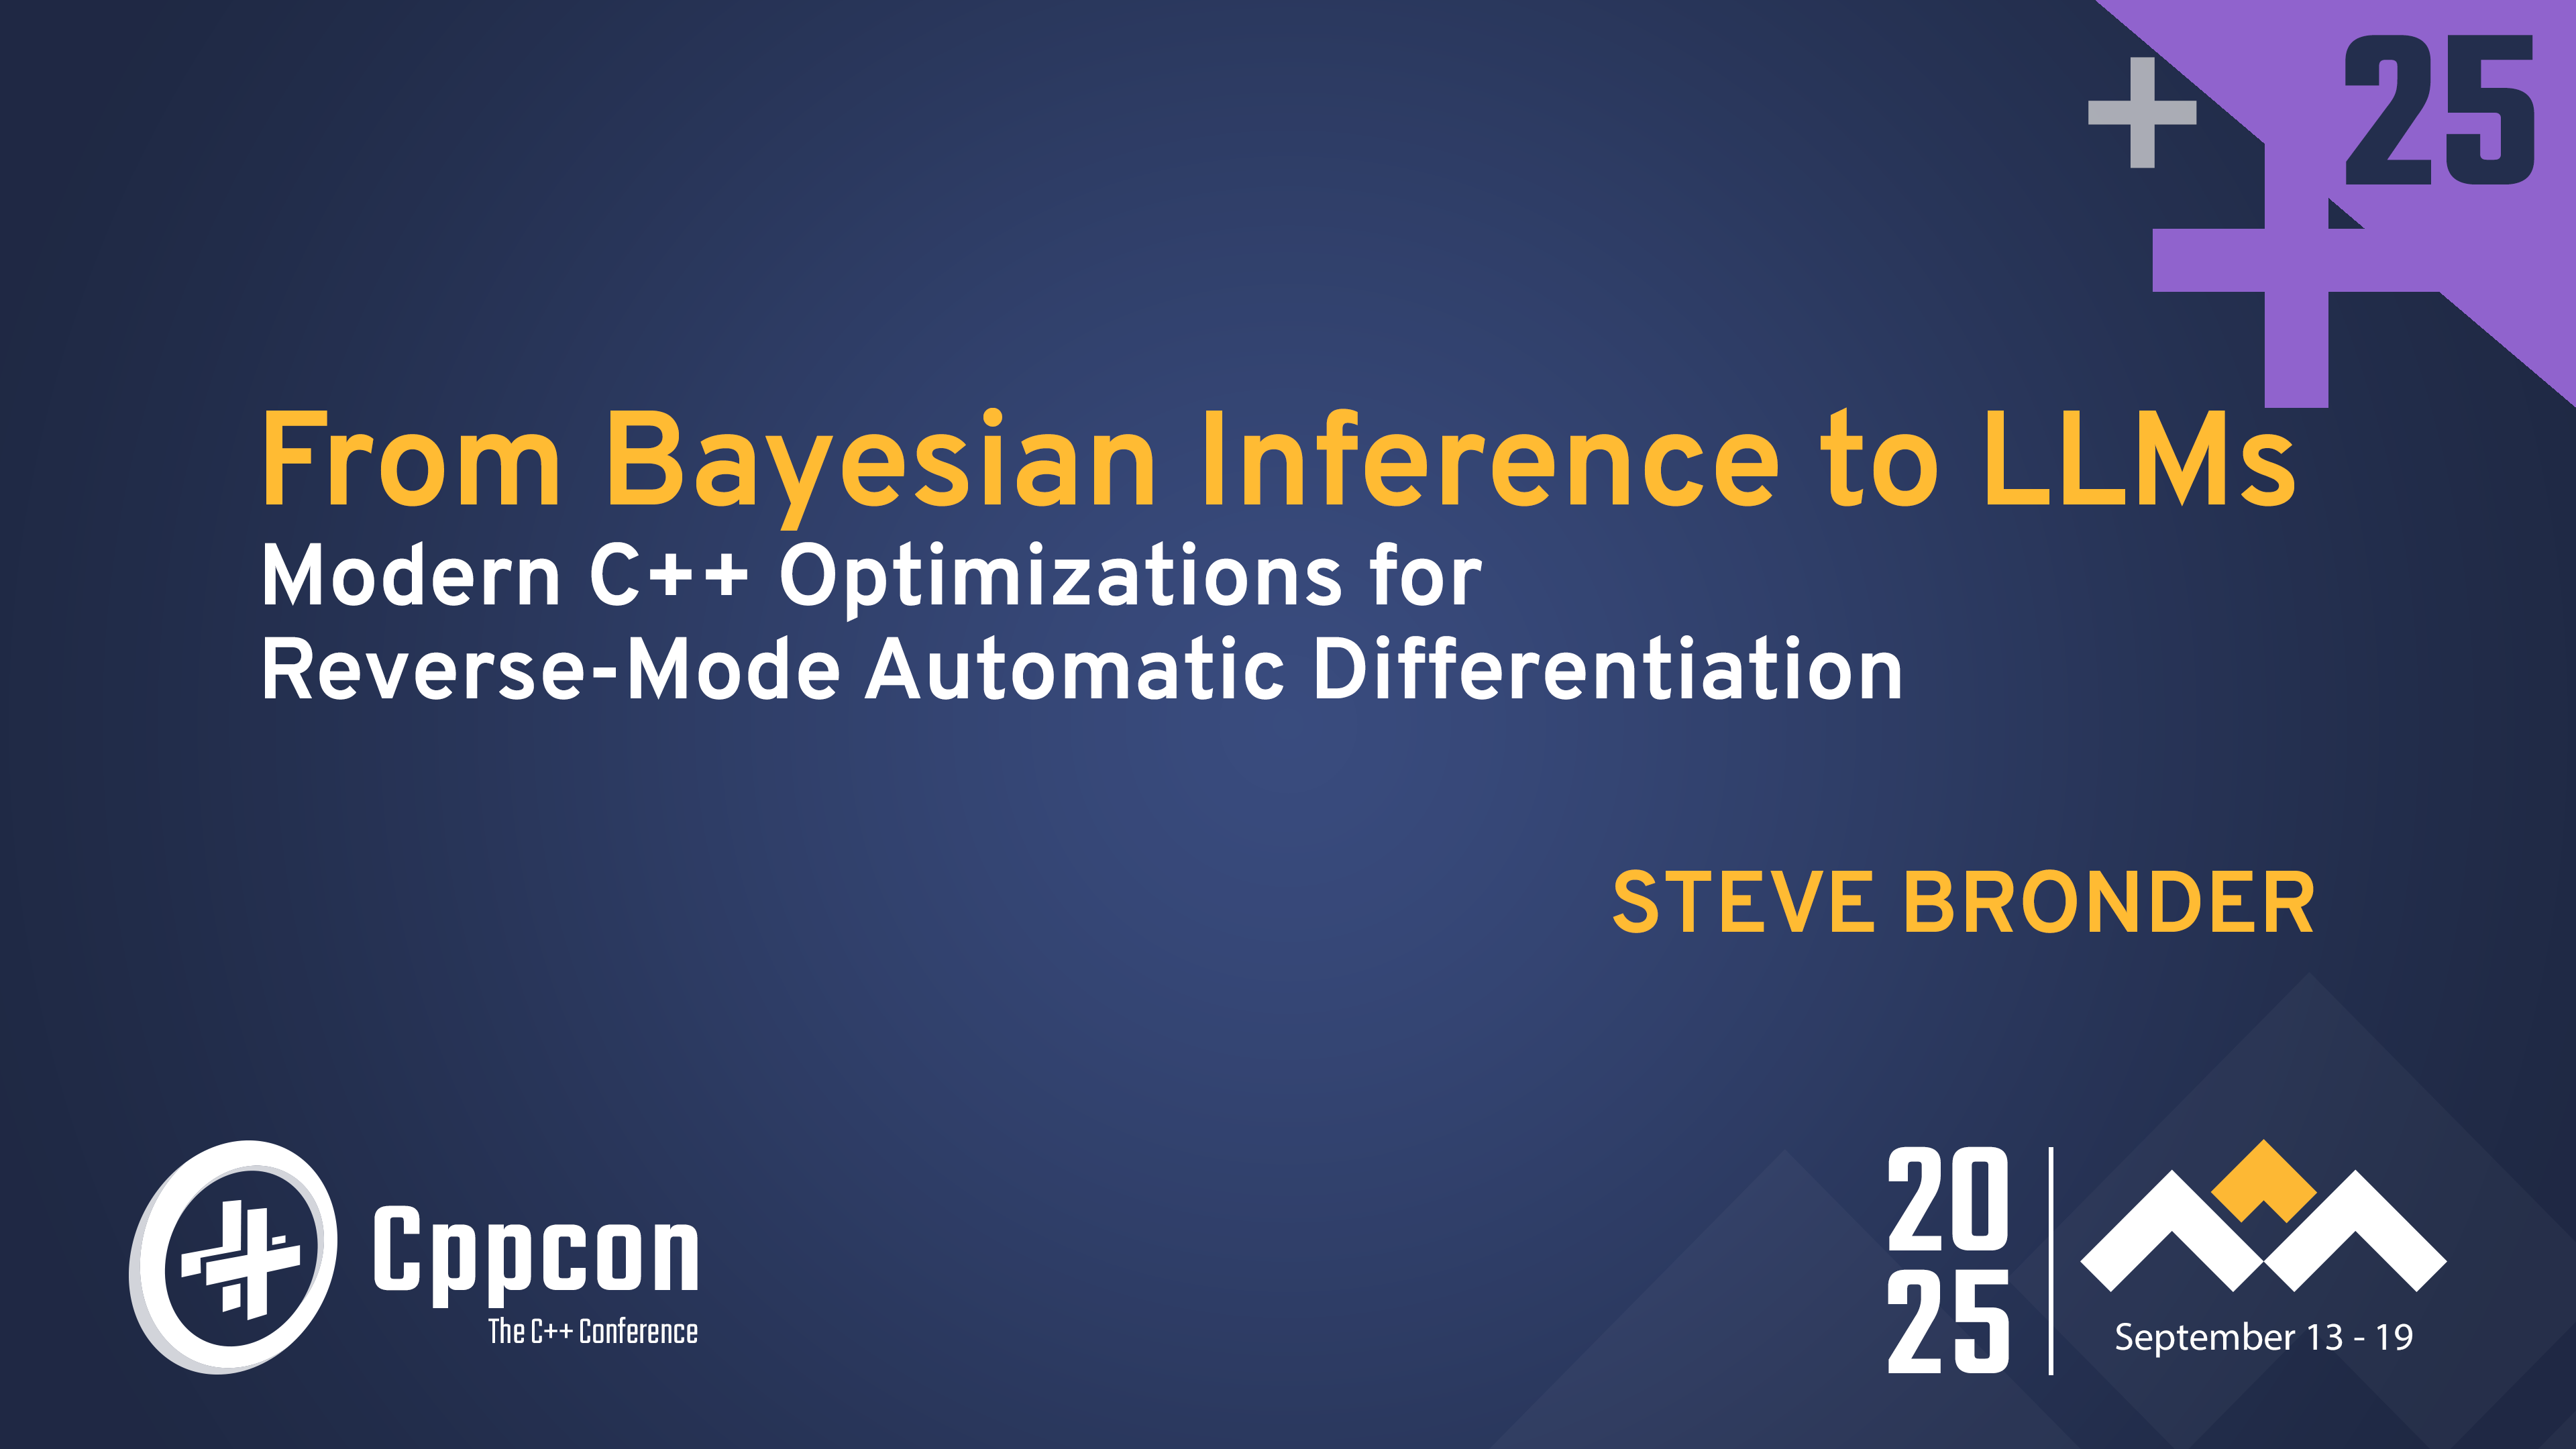
\includegraphics[keepaspectratio,
                         width=\paperwidth,
                         height=\paperheight]{img/title_card.png}
      };
      % Logo on top, bottom-left
      \node[anchor=south west, xshift=1em, yshift=1em]
        at (current page.south west) {
          
\includegraphics[width=2cm]{img/flatiron.png}
      };
    \end{tikzpicture}
  \end{frame}
}
\note{..}

\begin{comment}

{ % all template changes are local to this group.
    \setbeamertemplate{navigation symbols}{}
    \begin{frame}<article:0>[plain]
        \begin{tikzpicture}[remember picture,overlay]
            \node[at=(current page.center)] {
                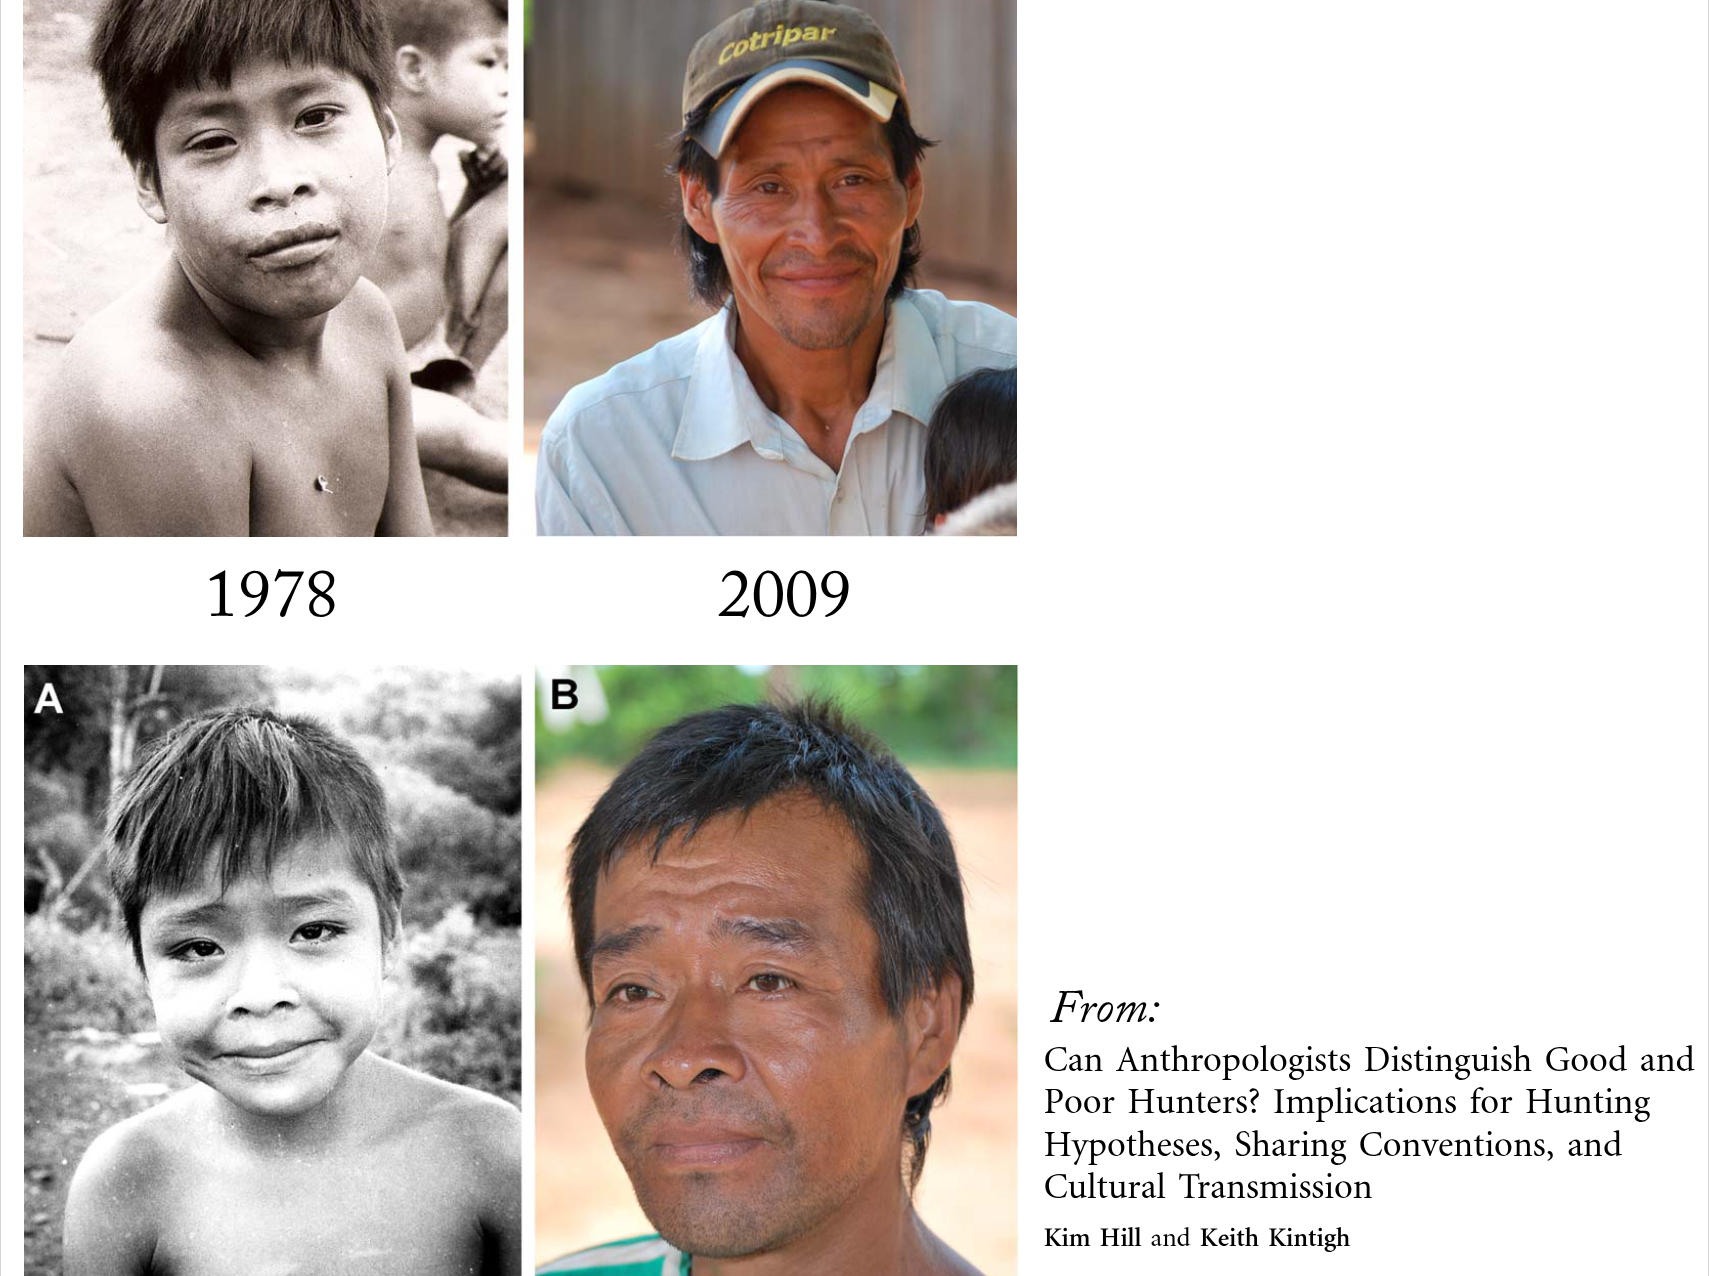
\includegraphics[keepaspectratio,
                                 width=\paperwidth,
                                 height=\paperheight]{img/mcel1.png}
            };
        \end{tikzpicture}
     \end{frame}
}

{ % all template changes are local to this group.
    \setbeamertemplate{navigation symbols}{}
    \begin{frame}<article:0>[plain]
        \begin{tikzpicture}[remember picture,overlay]
            \node[at=(current page.center)] {
                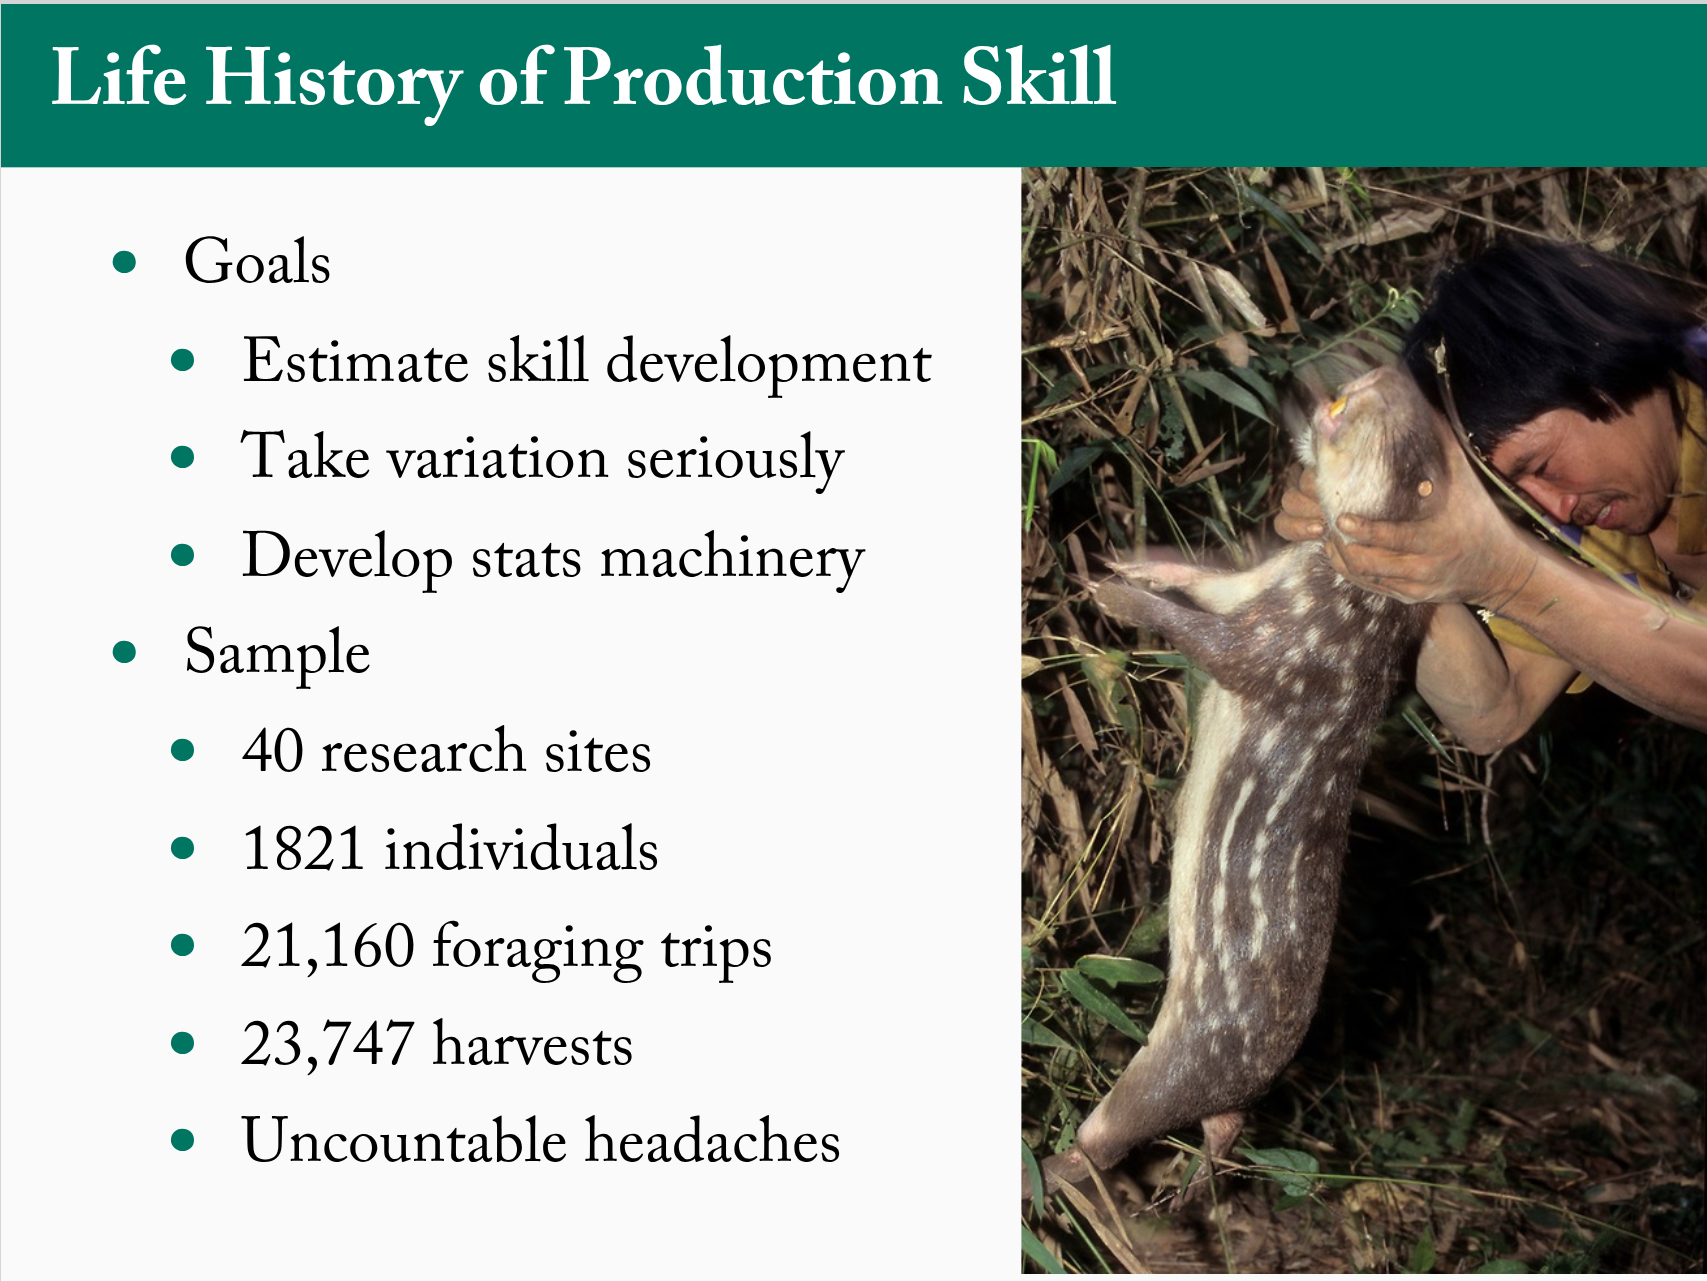
\includegraphics[keepaspectratio,
                                 width=\paperwidth,
                                 height=\paperheight]{img/mcel2.png}
            };
        \end{tikzpicture}
     \end{frame}
}

{ % all template changes are local to this group.
    \setbeamertemplate{navigation symbols}{}
    \begin{frame}<article:0>[plain]
        \begin{tikzpicture}[remember picture,overlay]
            \node[at=(current page.center)] {
                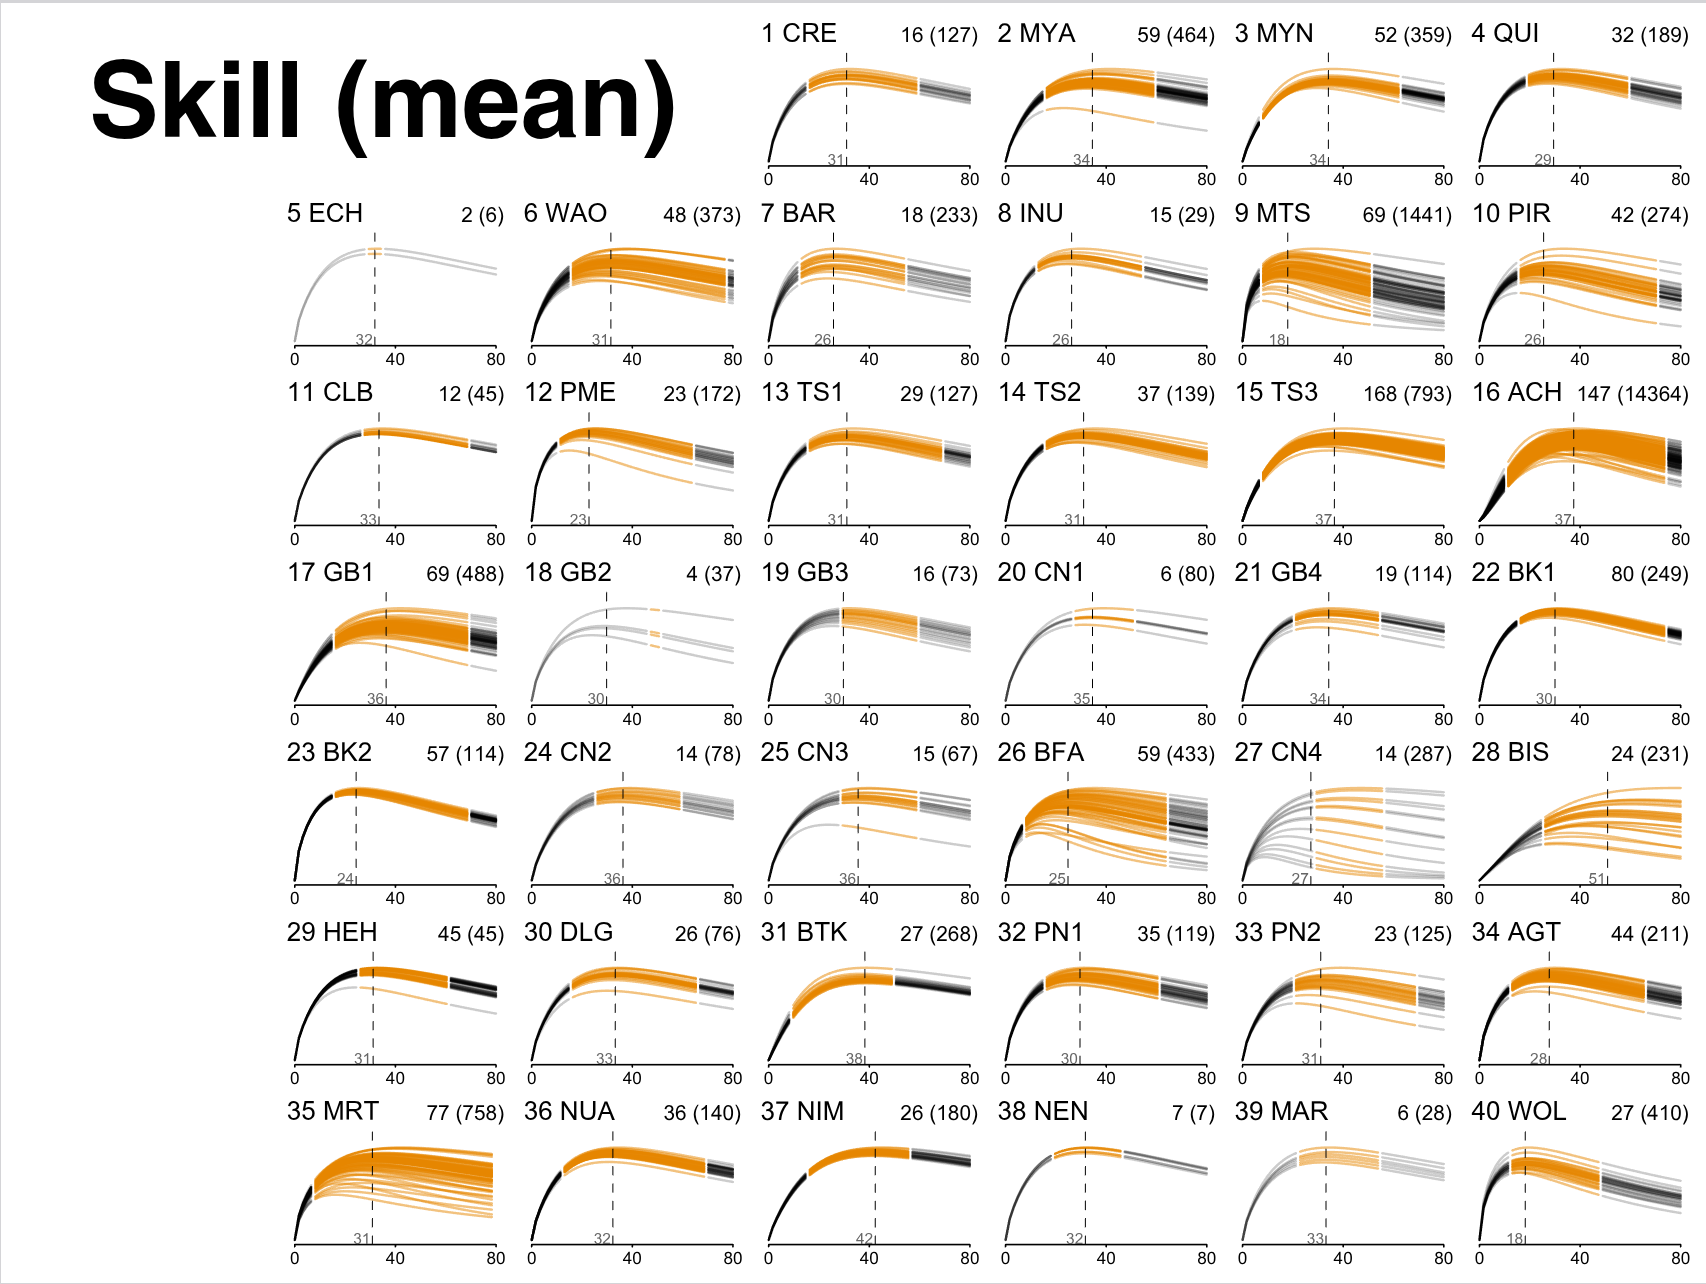
\includegraphics[keepaspectratio,
                                 width=\paperwidth,
                                 height=\paperheight]{img/mcel3.png}
            };
        \end{tikzpicture}
     \end{frame}
}
\end{comment}
\begin{frame}{Estimating COVID Infection Rates For Policy}
\begin{figure}
\centerline{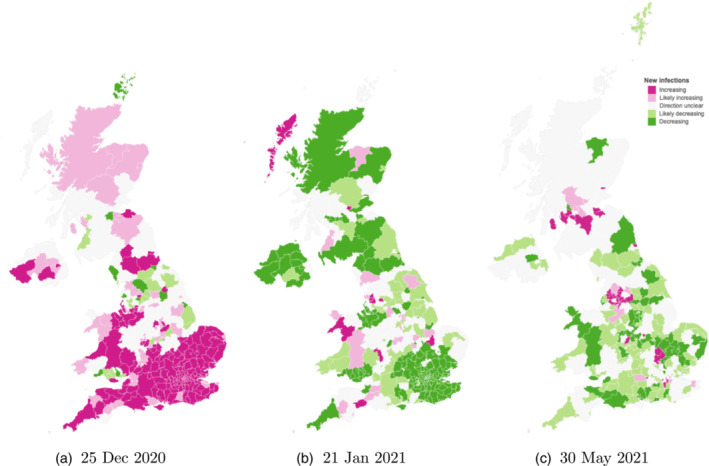
\includegraphics[scale=.5]{img/covid_uk.jpg}}
\caption{Probability of epidemic growth by local area}
\label{fig-covid}
\end{figure}
\end{frame}
\note{Go to ChatGPT. Autodiff is the mitochondria of machine learning. AD allows for efficient estimation of many statistical models.}


\begin{frame}{What is Automatic Differentiation?}
Automatically compute exact gradients by treating a program as a graph of elementary operations and applying the chain rule on that graph
\end{frame}
\note{
Reverse-mode automatic differentiation (AD) lets us get derivatives of a program's output with respect to its inputs without doing algebra by hand. Imagine the code as a computational graph of simple ops (add, multiply, sin, etc.). In the forward pass, we execute the code normally, get the output, and save intermediate results. Then we do a backward pass effectively running the chain rule on the graph from the output back to the inputs. This two-pass strategy is what powers deep learning frameworks (it's basically backpropagation), and it efficiently produces gradients even for complex code.
}

\begin{frame}{What is a gradient?}
Ex: Newton's root finding method
\begin{equation*}
    x_{n+1} = x_n - \frac{f\left(x_n\right)}{f_x'\left(x_{n}\right)}
\end{equation*}
find $f(x)=y$ where $y=0$
\end{frame}
\note{
\begin{itemize}
\item[-] Note that $f_x'$ is the gradient of $f$ with respect to $x$
\item[] How do we estimate solutions for equations? A simple method is the newton method.
\item[] Why are gradients useful? We use gradients to solve
\item[] For models we want to estimate parameter values. Change the slide here so that we show how to solve for parameters using Newton's method
\end{itemize}
}

\begin{frame}{What is a gradient?}
\begin{align}
    f(x) &= x^3 + x^2 + x\\
    f_x'(x) &= 3x^2 + 2x + 1
\end{align}
\centering
% Actual 266
\animategraphics[loop,controls,scale=0.12]{6}{gif/frame}{0001}{020}
\end{frame}
\note{
  \begin{itemize}
    \item[] The gradient tells us
    \item[-] The direction the function increases most quickly from $x_n$
    \item[-] The rate of increase of the function at $x_n$
  \end{itemize}
}

\begin{frame}{Why use Automatic Differentiation?}
\begin{itemize}
    \item[-] Hamiltonian Monte Carlo:
    \begin{itemize}
    \item[] $\frac{dp}{dt}=\nabla_\theta\log p(\theta|y)$
    \end{itemize}
    \item[-] BFGS:
    \begin{itemize}
    \item[] $s_k=-H_k \nabla_\theta f(\theta_k)$
    \end{itemize}
    \item[-] Stochastic Gradient Descent:
    \begin{itemize}
    \item[] $\theta_{t+1}=\theta_t−\eta\nabla_\theta L(\theta_t;x_t)$
    \end{itemize}
\end{itemize}
\end{frame}
\note{
\begin{itemize}
\item[] Hamiltonian Monte Carlo:
\begin{itemize}
  \item[-] Updates the momentum $p$ using the (negative) gradient of the log posterior—i.e., the deterministic “force” driving the Hamiltonian dynamics.
\end{itemize}
\item[] BFGS:
\begin{itemize}
  \item[-] Forms the search step $s_k$ as a quasi-Newton descent direction by preconditioning the gradient with the current inverse-Hessian estimate $H_k$.
\end{itemize}
\item[] Stochastic Gradient Descent:
\begin{itemize}
  \item[-] Updates parameters by stepping $\theta$ a learning-rate $\eta$ in the direction opposite the stochastic gradient of the loss evaluated on $x_t$.
\end{itemize}
\end{itemize}
}

\begin{frame}{Why use Automatic Differentiation?}
Choices:
    \begin{itemize}
        \item[-] Write by hand
        \item[-] finite difference,
        \item[-] symbolic differentiation
        \item[-] spectral differentiation
        \item[-] automatic differentiation
    \end{itemize}
\end{frame}
\note{..}


\begin{frame}{Why use Automatic Differentiation?}

\tiny
\begin{align*}
&\underbrace{p\!\left(
\boldsymbol{\theta} \,\big|\, \mathbf y
\right)}_{\textbf{posterior}}
\;\propto\;
\prod_{i=1}^{N}
\Bigg\{
\sum_{\mathbf z_i \in \{1,2,3\}^{T_i}}
\!\Bigg[
\underbrace{\pi_{z_{i,1}}\prod_{t=2}^{T_i}\Pi_{z_{i,t-1},\,z_{i,t}}}_{\text{3-state HMM prior}}
\;
\prod_{t=1}^{T_i}
\underbrace{\mathcal N\!\Big(
y_{i,t}\,\Big|\,\eta_{i,t},\,\sigma_{z_{i,t}}^{2}
\Big)}_{\text{state-dependent emission}}
\Bigg]
\Bigg\}
\\[-2pt]
&\text{where}\quad
\eta_{i,t}
=\underbrace{\mathbf x_{i,t}^{\!\top}\boldsymbol\beta}_{\text{fixed}}
+\underbrace{\mathbf z^{(G)}_{i,t}{}^{\!\top}\mathbf b_{g[i]}
+\mathbf z^{(C)}_{i,t}{}^{\!\top}\mathbf c_{c[i]}
+u_{g[i]}}_{\text{crossed random effects}}
+\underbrace{f(t_{i,t})}_{\text{GP}}
+\underbrace{\mu_{z_{i,t}}
+\mathbf r_{z_{i,t}}^{\!\top}\mathbf w_i}_{\text{state-specific offset + slope}}
,\qquad z_{i,t}\in\{1,2,3\}.
\\[4pt]
&
p(\mathbf f\mid\boldsymbol\psi)
=
(2\pi)^{-T/2}\,|\mathbf K|^{-1/2}\;
\exp\!\Big(-\tfrac12\,\mathbf f^{\!\top}\mathbf K^{-1}\mathbf f\Big),
\\[-2pt]
&
\mathbf K
=\sigma_f^{2}\Big(\mathbf K_{\text{LP}}(\ell,p,\lambda)\;+\;\rho\,\mathbf K_{\text{SE}}(\tilde\ell)\Big)
+\sigma_n^{2}\mathbf I,\quad
\big[\mathbf K_{\text{LP}}\big]_{t t\,'}
=\exp\!\left(
-\frac{(t-t')^{2}}{2\ell^{2}}
-\frac{2\sin^{2}\!\big(\pi|t-t'|/p\big)}{\lambda^{2}}
\right),
\\[-2pt]
&
\big[\mathbf K_{\text{SE}}\big]_{t t'}
=
\exp\!\left(-\frac{(t-t')^{2}}{2\tilde\ell^{2}}\right),
\qquad
\mathbf K=\mathbf L_K\mathbf L_K^{\!\top}
\;\Rightarrow\;
\log|\mathbf K|=2\sum_{j=1}^{T}\log \big((\mathbf L_K)_{jj}\big).
\\[6pt]
&\textbf{Hierarchical mixed effects (non-centered, LKJ prior):}
\\[-2pt]
&\qquad
\mathbf b_{g}=\big(\mathbf I_{p_G}\otimes\operatorname{diag}(\boldsymbol\tau_b)\,\mathbf L_R\big)\,\tilde{\mathbf b}_{g},
\;\;
\tilde{\mathbf b}_{g}\sim\mathcal N(\mathbf 0,\mathbf I),
\;\;
\mathbf c_{c}=\operatorname{diag}(\boldsymbol\tau_c)\,\tilde{\mathbf c}_{c},
\;\;
\tilde{\mathbf c}_{c}\sim\mathcal N(\mathbf 0,\mathbf I),
\\[-2pt]
&\qquad
\operatorname{LKJ}_{p_G}(\eta)\ \text{prior on}\ \mathbf R,\quad
\mathbf L_R\mathbf L_R^{\!\top}=\mathbf R,
\quad
\boldsymbol\tau_b\sim\prod_{j=1}^{p_G}\text{Half-}t_{\nu_b}(0,s_b),
\quad
\boldsymbol\tau_c\sim\prod_{j=1}^{p_C}\text{Half-}t_{\nu_c}(0,s_c),
\\[-2pt]
&\qquad
u_g\sim\mathcal N(0,\sigma_u^2).
\end{align*}
\end{frame}
\note{Move from this slide quickly}

\begin{frame}{Why use Automatic Differentiation?}
\begin{itemize}
\item[-] I do not wish to write those gradients by hand
\pause
\note{..}
\item Instead of N finite differences, just a forward and backward pass
\pause
\note{..}
\item Allows for unknown length while and for loops
\pause
\note{..}
\item Accurate to floating point precision
\pause
\end{itemize}
\end{frame}

\begin{comment}
RIP Bob said no :(
\begin{frame}{How Fast is AutoDiff?}
\begin{figure}
\centerline{
\includegraphics[scale=.5]{img/mocking-spongebob.jpg}}
\caption{AuToDiFf rUnS iN $\Theta(C(f))$ TiMe}
\label{fig-spongebob}
\end{figure}
\end{frame}
\end{comment}

\begin{frame}{Implementation Matters!}
\begin{figure}
\centerline{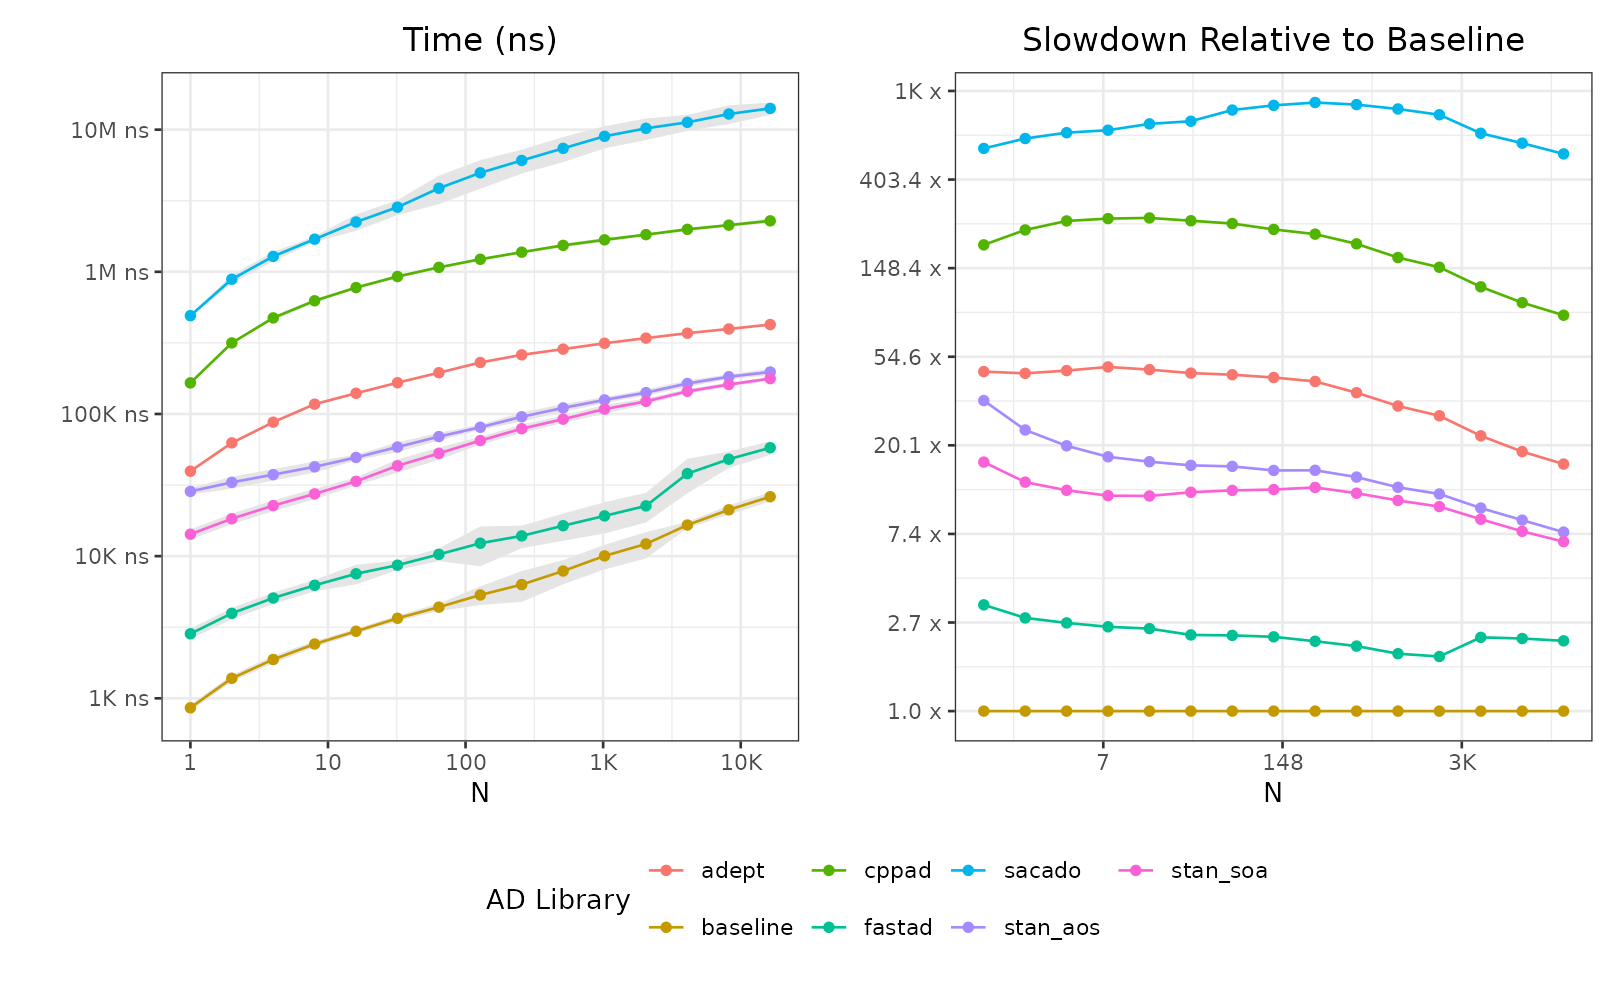
\includegraphics[scale=.5]{img/linux_regression_plot.png}}
\caption{Benchmark for $f$ and $f\,'$ given $f(y) = N(y | X\theta,\sigma)$}
\label{fig-mac-red-bench}
\end{figure}
\end{frame}
\note{..}

\begin{frame}{Goal of this talk}
\begin{itemize}
    \item How Reverse Mode Automatic Differentiation works
    \item Performance of high throughput memory intensive programs
    \item How modern C++ has led to cleaner and more efficient AD
\end{itemize}
\end{frame}
\note{Let $v_k$ be the sequence of intermediate expressions for the input $x$ and output $z$ and let $v_K = z$ and $v_1 = x; v_0 = y$. Let $\overline{v}_k$ be the partial gradient of the kth intermediate step. Then we can apply the chain rule to each intermediate step to get the partial gradient.}


\begin{frame}[fragile]{What is Automatic Differentiation?}
\begin{itemize}
  \item AD computes gradients of a program by applying the chain rule to its subexpressions.
%  \item Given a function $f$ with inputs $x\in\mathbb{R}^n$ and outputs $z\in \mathbb{R}^m$ we want to "calculate the Jacobian $J\,$" with size $(m, n)$
\end{itemize}
\begin{align*}
f\,(x, y) &= \log(x\cdot y)\\
g(x, y) &= x \cdot y \\
h(u) &= \log(u) \\
f\,(x,y) &= h\,\!\big(g(x,y)\big) \\
\end{align*}
\end{frame}
\note{
  \begin{itemize}
    \item Emphasize: AD is mechanical chain rule over the executed program, not symbolic math or numeric differencing.
    \item Automatic Differentiation can do higher order partials, but here we just focus on the first order
    \item Now we rewrite $f$ in terms of $h$ and $g$
  \end{itemize}
}

\begin{frame}[fragile]{What is Automatic Differentiation?}
\begin{itemize}
  \item AD computes gradients of a program by applying the chain rule to its subexpressions.
%  \item Given a function $f$ with inputs $x\in\mathbb{R}^n$ and outputs $z\in \mathbb{R}^m$ we want to "calculate the Jacobian $J\,$" with size $(m, n)$
\end{itemize}
\begin{align*}
f\,(x,y) &= h\,\!\big(g(x,y)\big) \\
g(x, y) &= x \cdot y \;& g_x\,'(x,y) = y \:\; g_y\,'(x,y) = x\\[2pt]
h(u) &= \log(u) \;& h_u'(u) = u^{-1}\\
\end{align*}
\vspace{-1cm}
\begin{align*}
f\,'_x(x,y)
  &= h'_g\!\big(g(x,y)\big)\,\cdot\, g\,'_x(x,y) \\
  &= \frac{1}{g(x, y)} \cdot y = \frac{1}{x}, \\[6pt]
f\,'_y(x,y)
  &= h'_g\!\big(g(x,y)\big)\,\cdot\, g\,'_y(x,y) \\
  &= \frac{1}{g(x, y)} \cdot x = \frac{1}{y}.
\end{align*}
%Automatic Differentiation can do higher order partials, but here we just focus on the first order
\end{frame}
\note{Emphasize: AD is mechanical chain rule over the executed program, not symbolic math or numeric differencing.}

\begin{frame}{Data Type: Expression Graph}
  Goal: Calculate the full gradient by accumulating partial gradients (adjoints) through the a graph of subexpressions.
\vspace{-1mm}
$$z = \log(x) \cdot y + \sin(x)$$

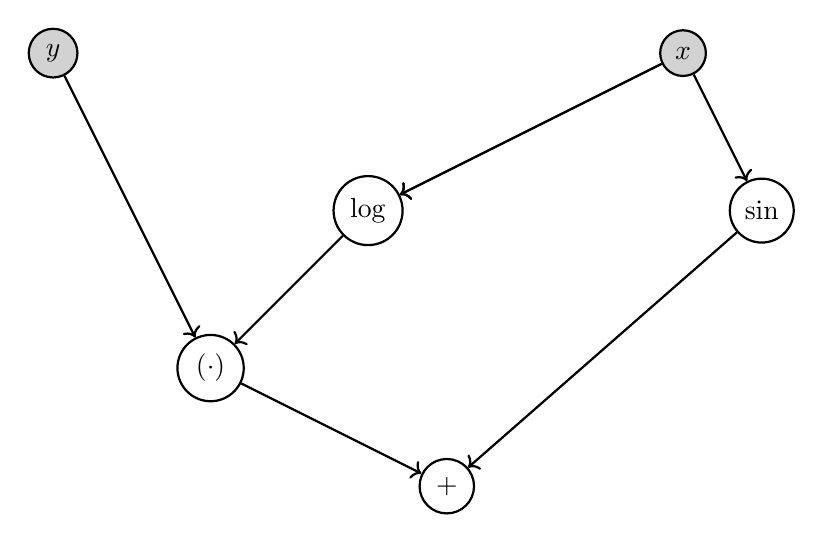
\begin{tikzpicture}
  [
    Round/.style={circle, draw=black!, fill=green!0, thick, minimum size=2mm},
    Red/.style={circle, draw=black!, fill=red!255, thick, minimum size=2mm},
    Yellow/.style={circle, draw=black!, fill=yellow!255, thick, minimum size=10mm},
    Gray/.style={circle, draw=black!, fill=gray!35, thick, minimum size=2mm}
  ]
  % Nodes
  \node[Gray] (v1) at(-8, 0) {$y$};
  \node[Gray] (v2) at(0, 0) {$x$};
  \node[Round] (v3) at(-4, -2) {$\log$};
  \node[Round] (v4) at(1, -2) {$\sin$};
  \node[Round] (v5) at(-6, -4) {$(\cdot)$};
  \node[Round] (v6) at(-3, -5.5) {$+$};

  % Lines
  \path [<-, draw, thick] (v5) -- (v1);
  \path [<-, draw, thick] (v3) -- (v2);
  \path [<-, draw, thick] (v4) -- (v2);
  \path [<-, draw, thick] (v3) -- (v2);
  \path [<-, draw, thick] (v6) -- (v4);
  \path [<-, draw, thick] (v6) -- (v5);
  \path [<-, draw, thick] (v5) -- (v3);

\end{tikzpicture}
\end{frame}
\note{
  \begin{itemize}
  \item[-] Each node of expression graph is an intermediate calculation we know the gradient of with respect to its inputs
  \item[-] For each node we compute a forward pass till we get to our end node
  \item[-] Once we reach our end node we can compute the reverse pass
  \end{itemize}
}


\begin{frame}{Expression Graph: Traversal}
\begin{equation*}
f(x, y) = \log(x)y + \sin(x)
\end{equation*}
\begin{figure}
  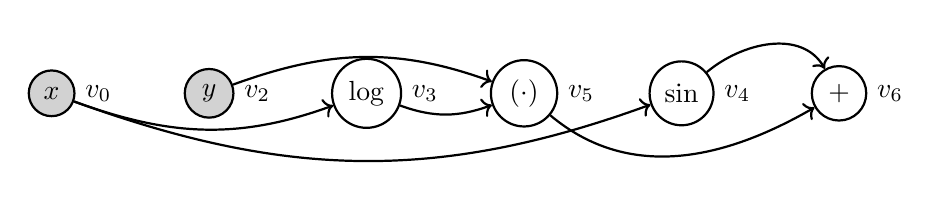
\begin{tikzpicture}
  [
    Round/.style={circle, draw=black!, fill=green!0, thick, minimum size=2mm},
    Red/.style={circle, draw=black!, fill=red!255, thick, minimum size=2mm},
    Yellow/.style={circle, draw=black!, fill=yellow!255, thick, minimum size=10mm},
    Gray/.style={circle, draw=black!, fill=gray!35, thick, minimum size=2mm}
  ]
  % Nodes
  \node[Gray, label=right:{$v_0$}] (v2) at(0, 0) {$x$};
  \node[Gray, label=right:{$v_2$}] (v1) at(2, 0) {$y$};
  \node[Round, label=right:{$v_3$}] (v3) at(4, 0) {$\log$};
  \node[Round, label=right:{$v_4$}] (v4) at(8, 0) {$\sin$};
  \node[Round, label=right:{$v_5$}] (v5) at(6, 0) {$(\cdot)$};
  \node[Round, label=right:{$v_6$}] (v6) at(10, 0) {$+$};


  % Lines
  \path [->, draw, thick] (v1) to[out=20,in=160] (v5);
  \path [->, draw, thick] (v2) to[out=-20,in=-160] (v3);
  \path [->, draw, thick] (v2) to[out=-20,in=-160] (v4);
  \path [->, draw, thick] (v3) to[out=-20,in=-160] (v5);
  \path [->, draw, thick] (v4) to[out=40,in=120] (v6);
  \path [->, draw, thick] (v5) to[out=320,in=210] (v6);

\end{tikzpicture}
  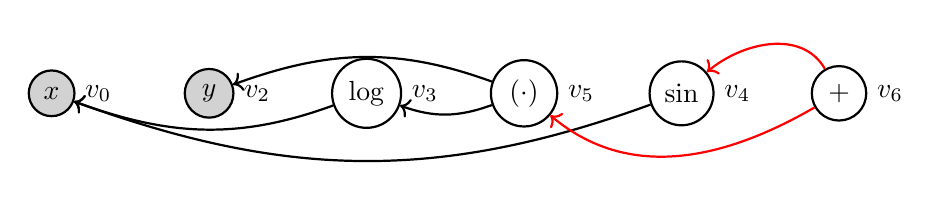
\begin{tikzpicture}
  [
    Round/.style={circle, draw=black!, fill=green!0, thick, minimum size=2mm},
    Red/.style={circle, draw=black!, fill=red!255, thick, minimum size=2mm},
    Yellow/.style={circle, draw=black!, fill=yellow!255, thick, minimum size=10mm},
    Gray/.style={circle, draw=black!, fill=gray!35, thick, minimum size=2mm}
  ]
  % Nodes
  \node[Gray, label=right:{$v_0$}] (v2) at(0, 0) {$x$};
  \node[Gray, label=right:{$v_2$}] (v1) at(2, 0) {$y$};
  \node[Round, label=right:{$v_3$}] (v3) at(4, 0) {$\log$};
  \node[Round, label=right:{$v_4$}] (v4) at(8, 0) {$\sin$};
  \node[Round, label=right:{$v_5$}] (v5) at(6, 0) {$(\cdot)$};
  \node[Round, label=right:{$v_6$}] (v6) at(10, 0) {$+$};


  % Lines
  \path [<-, draw, thick] (v1) to[out=20,in=160] (v5);
  \path [<-, draw, thick] (v2) to[out=-20,in=-160] (v3);
  \path [<-, draw, thick] (v2) to[out=-20,in=-160] (v4);
  \path [<-, draw, thick] (v3) to[out=-20,in=-160] (v5);
  \path [<-, draw=red, thick] (v4) to[out=40,in=120] (v6);
  \path [<-, draw=red, thick] (v5) to[out=320,in=210] (v6);

\end{tikzpicture}
\caption{Topological sort of expression graph}
\end{figure}
\end{frame}
\note{
  \begin{itemize}
  \item[-] We can do a Topological sort on the graph and traverse it this way
  \item[-] This is how we should execute the program linearly on a thread
  \end{itemize}
}

\begin{frame}{Expression Graph: Node}
 For Reverse Mode AD, each node performs two functions.
\begin{itemize}
 \item Forward Pass:
 \begin{equation*}
     z = f\,(x, y)
 \end{equation*}
 \item Reverse Pass: Given $z$'s adjoint (partial gradient) $\overline{z}$
 \\Calculate the local adjoint-Jacobian update for $x$ and $y$.
 \begin{equation*}
 chain(\overline{z}, y, x) =
 \begin{cases}
  \overline{y} \pluseq \overline{z} \cdot z_{y}\,'\\
  \overline{x} \pluseq \overline{z} \cdot z_{x}\,'
 \end{cases}
 \end{equation*}
\end{itemize}
\end{frame}
\note{
\begin{itemize}
\item[] Adjoint = local gradient
\begin{itemize}
\item[-] Each node in the graph holds an adjoint value, which is the partial derivative of the final output with respect to that node's value. It accumulates all contributions of that node to the output's gradient.
\end{itemize}
\item[] Backpropagation (chain rule):
\begin{itemize}
  \item[-] During the backward pass, each operation uses its adjoint and the operation's local derivative to add to its input nodes' adjoints. This is how gradients flow backward through the graph
\end{itemize}
\end{itemize}
}

\begin{frame}[fragile]{Pseudocode for AutoDiff}
\begin{minted}{C++}
// compute and store node.value
struct node {
  double val;
  double adj;
  virtual void chain() {}
};
node x = 2.0;
node y = 3.0;
// Forward pass calculated here
auto e_graph = log(x) * y + sin(x);
// Calculate reverse pass
e_graph.end().adj = 1.0;
for (auto& node : e_graph | std::views::reverse) {
    (*node)->chain();
}
assert(y.adj == 1.2103);
assert(x.adj == 0.2516);
\end{minted}
\end{frame}

\begin{comment}
\begin{frame}{Forward Pass}
\vspace{-1mm}
$$z = \log(x*y)$$

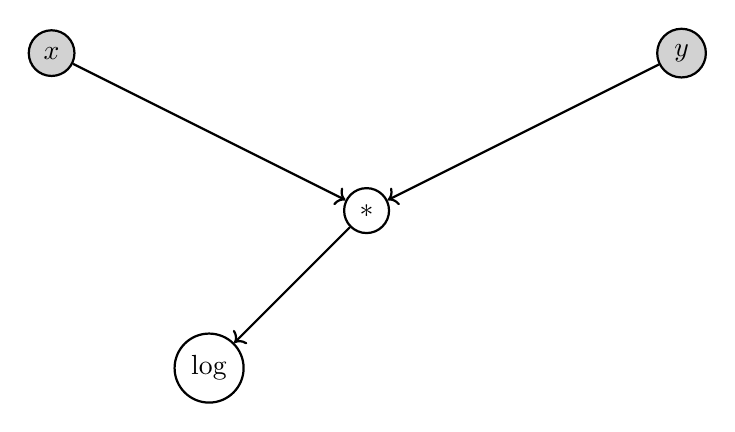
\begin{tikzpicture}
  [
    Round/.style={circle, draw=black!, fill=green!0, thick, minimum size=2mm},
    Red/.style={circle, draw=black!, fill=red!255, thick, minimum size=2mm},
    Yellow/.style={circle, draw=black!, fill=yellow!255, thick, minimum size=10mm},
    Gray/.style={circle, draw=black!, fill=gray!35, thick, minimum size=2mm}
  ]
  % Nodes
  \node[Gray] (v0) at(0, 0) {$y$};
  \node[Gray] (v1) at(-8, 0) {$x$};
  \node[Round] (v2) at(-4, -2) {$*$};
  \node[Round] (v3) at(-6, -4) {$\log$};

  % Lines
  \path [<-, draw, thick] (v2) -- (v0);
  \path [<-, draw, thick] (v2) -- (v1);
  \path [<-, draw, thick] (v3) -- (v2);

\end{tikzpicture}
\end{frame}

\begin{frame}{Forward Pass}
\vspace{-1mm}
$$z = \log(\mathcolor{red}{x} \cdot \mathcolor{red}{y})$$

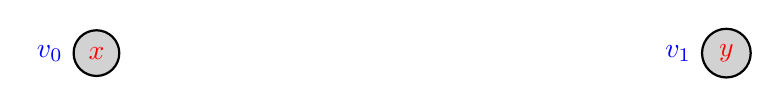
\begin{tikzpicture}
  [
    Round/.style={circle, draw=black!, fill=green!0, thick, minimum size=2mm},
    Red/.style={circle, draw=black!, fill=red!255, thick, minimum size=2mm},
    Yellow/.style={circle, draw=black!, fill=yellow!255, thick, minimum size=10mm},
    Gray/.style={circle, draw=black!, fill=gray!35, thick, minimum size=2mm}
  ]
  % Nodes
  \node[Gray, label=left:{\textcolor{blue}{$v_1$}}] (v0) at(0, 0) {$\mathcolor{red}{y}$};

  \node[Gray, label=left:{\textcolor{blue}{$v_0$}}] (v1) at(-8, 0) {$\mathcolor{red}{x}$};

\end{tikzpicture}
\end{frame}

\begin{frame}{Forward Pass}
\vspace{-1mm}
$$z = \log(x\mathcolor{red}{\cdot}y)$$

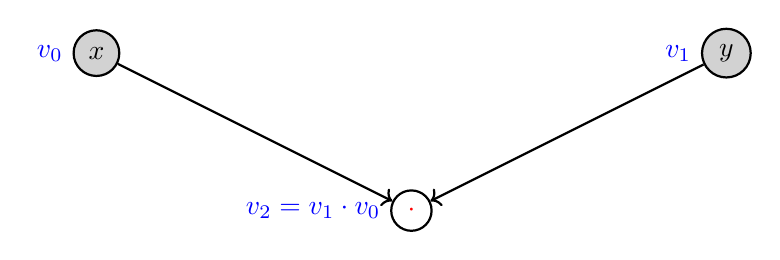
\begin{tikzpicture}
  [
    Round/.style={circle, draw=black!, fill=green!0, thick, minimum size=2mm},
    Red/.style={circle, draw=black!, fill=red!255, thick, minimum size=2mm},
    Yellow/.style={circle, draw=black!, fill=yellow!255, thick, minimum size=10mm},
    Gray/.style={circle, draw=black!, fill=gray!35, thick, minimum size=2mm}
  ]
  % Nodes
  \node[Gray, label=left:{\textcolor{blue}{$v_1$}}] (v0) at(0, 0) {$y$};

  \node[Gray, label=left:{\textcolor{blue}{$v_0$}}] (v1) at(-8, 0) {$x$};

  \node[Round, label=left:{\textcolor{blue}{$v_2 = v_1 \cdot v_0$}}] (v2) at(-4, -2) {$\mathcolor{red}{\cdot}$};


  % Lines
  \path [<-, draw, thick] (v2) -- (v0);
  \path [<-, draw, thick] (v2) -- (v1);

\end{tikzpicture}
\end{frame}

\begin{frame}{Forward Pass}
\vspace{-1mm}
$$z = \mathcolor{red}{\log}(x\cdot y)$$
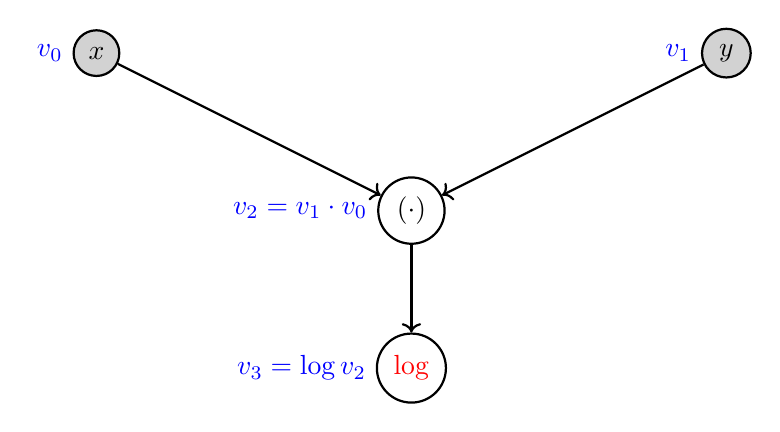
\begin{tikzpicture}
  [
    Round/.style={circle, draw=black!, fill=green!0, thick, minimum size=2mm},
    Red/.style={circle, draw=black!, fill=red!255, thick, minimum size=2mm},
    Yellow/.style={circle, draw=black!, fill=yellow!255, thick, minimum size=10mm},
    Gray/.style={circle, draw=black!, fill=gray!35, thick, minimum size=2mm}
  ]
  % Nodes
  \node[Gray, label=left:{\textcolor{blue}{$v_1$}}] (v0) at(0, 0) {$y$};
  \node[Gray, label=left:{\textcolor{blue}{$v_0$}}] (v1) at(-8, 0) {$x$};
  \node[Round, label=left:{\textcolor{blue}{$v_2 = v_1 \cdot v_0$}}] (v2) at(-4, -2) {$(\cdot)$};
  \node[Round, label=left:{\textcolor{blue}{$v_3 = \log{v_2}$}}] (v3) at(-4, -4) {$\mathcolor{red}{\log}$};
  % Lines
  \path [<-, draw, thick] (v2) -- (v0);
  \path [<-, draw, thick] (v2) -- (v1);
  \path [<-, draw, thick] (v3) -- (v2);
\end{tikzpicture}
\end{frame}

\begin{frame}{How do we calculate the adjoint Jacobian?}
Let $\overline{v}_i$ be the adjoint of $v_i$

\begin{equation*}
    \overline{v}_i = \fracp{v_{i + 1}}{v_i} \overline{v}_{i + 1}
\end{equation*}
Automatic Differentiation only needs the partials of the intermediates
\begin{align*}
    v_2 &= v_1 \cdot v_0 &\: \fracp{v_2}{v_1}&=v_0, \fracp{v_2}{v_0}=v_1\\
    v_3 &= \log(v_2) &\: \fracp{v_3}{v_2}&=\frac{1}{v_2}\\
\end{align*}
\end{frame}

\begin{frame}{Reverse Pass}
\vspace{-1mm}
$$z = \mathcolor{red}{\log(x\cdot y)}$$
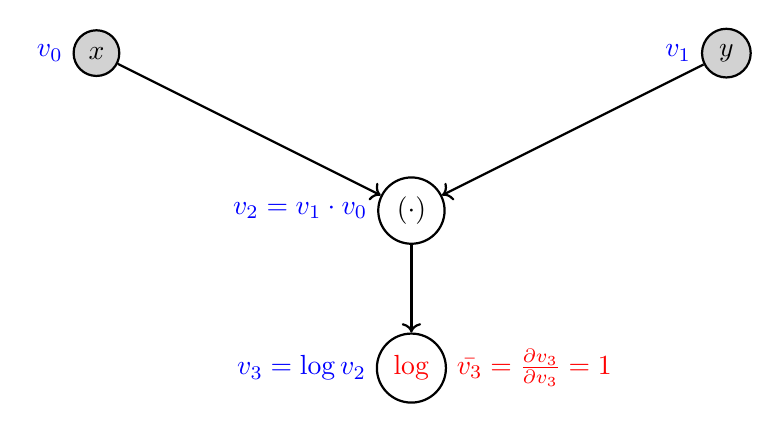
\begin{tikzpicture}
  [
    Round/.style={circle, draw=black!, fill=green!0, thick, minimum size=2mm},
    Red/.style={circle, draw=black!, fill=red!255, thick, minimum size=2mm},
    Yellow/.style={circle, draw=black!, fill=yellow!255, thick, minimum size=10mm},
    Gray/.style={circle, draw=black!, fill=gray!35, thick, minimum size=2mm}
  ]
  % Nodes
  \node[Gray, label=left:{\textcolor{blue}{$v_1$}}] (v0) at(0, 0) {$y$};
  \node[Gray, label=left:{\textcolor{blue}{$v_0$}}] (v1) at(-8, 0) {$x$};
  \node[Round, label=left:{\textcolor{blue}{$v_2 = v_1 \cdot v_0$}}] (v2) at(-4, -2) {$(\cdot)$};
  \node[Round, label=left:{\textcolor{blue}{$v_3 = \log{v_2}$}},
    label=right:{\textcolor{red}{$\adj{v_3}=\pp{v_3}{v_3}=1$}}] (v3) at(-4, -4) {$\mathcolor{red}{\log}$};
  % Lines
  \path [<-, draw, thick] (v2) -- (v0);
  \path [<-, draw, thick] (v2) -- (v1);
  \path [<-, draw, thick] (v3) -- (v2);
\end{tikzpicture}
\end{frame}

\begin{frame}{Reverse Pass}
\vspace{-1mm}
$$z = \log(\mathcolor{red}{x\cdot y})$$
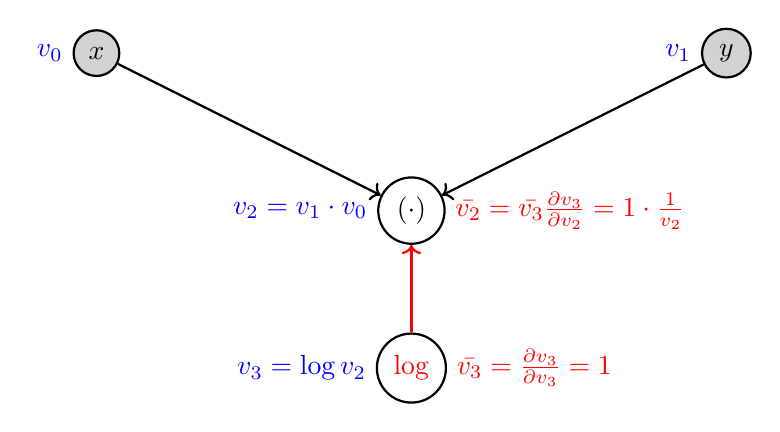
\begin{tikzpicture}
  [
    Round/.style={circle, draw=black!, fill=green!0, thick, minimum size=2mm},
    Red/.style={circle, draw=black!, fill=red!255, thick, minimum size=2mm},
    Yellow/.style={circle, draw=black!, fill=yellow!255, thick, minimum size=10mm},
    Gray/.style={circle, draw=black!, fill=gray!35, thick, minimum size=2mm}
  ]
  % Nodes
  \node[Gray, label=left:{\textcolor{blue}{$v_1$}}] (v0) at(0, 0) {$y$};
  \node[Gray, label=left:{\textcolor{blue}{$v_0$}}] (v1) at(-8, 0) {$x$};
  \node[Round, label=left:{\textcolor{blue}{$v_2 = v_1 \cdot v_0$}},
    label=right:{\textcolor{red}{$\adj{v_2}=\adj{v_3}\pp{v_3}{v_2}=1\cdot \frac{1}{v_2}$}}] (v2) at(-4, -2) {$(\cdot)$};
  \node[Round, label=left:{\textcolor{blue}{$v_3 = \log{v_2}$}},
    label=right:{\textcolor{red}{$\adj{v_3}=\pp{v_3}{v_3}=1$}}] (v3) at(-4, -4) {$\mathcolor{red}{\log}$};
  % Lines
  \path [<-, draw, thick] (v2) -- (v0);
  \path [<-, draw, thick] (v2) -- (v1);
  \path [->, draw=red, thick] (v3) -- (v2);
\end{tikzpicture}
\end{frame}

\begin{frame}{Reverse Pass}
\vspace{-1mm}
$$z = \log(x\cdot \mathcolor{red}{y})$$
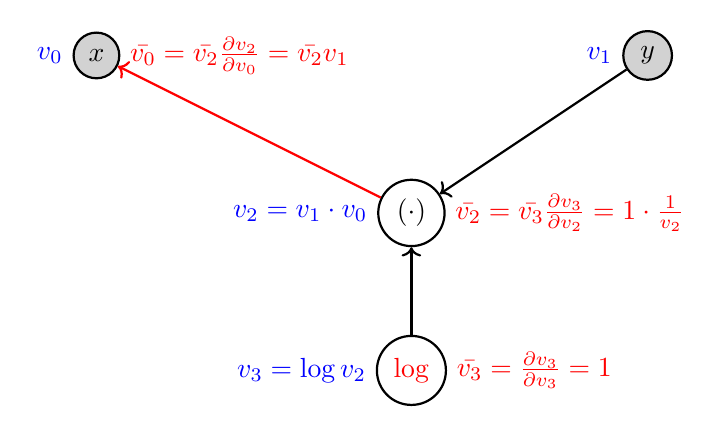
\begin{tikzpicture}
  [
    Round/.style={circle, draw=black!, fill=green!0, thick, minimum size=2mm},
    Red/.style={circle, draw=black!, fill=red!255, thick, minimum size=2mm},
    Yellow/.style={circle, draw=black!, fill=yellow!255, thick, minimum size=10mm},
    Gray/.style={circle, draw=black!, fill=gray!35, thick, minimum size=2mm}
  ]
  % Nodes
  \node[Gray, label=left:{\textcolor{blue}{$v_1$}}] (v0) at(-1, 0) {$y$};
  \node[Gray, label=left:{\textcolor{blue}{$v_0$}},
    label=right:{\textcolor{red}{$\adj{v_0}=\adj{v_2}\pp{v_2}{v_0}=\adj{v_2}v_1$}}] (v1) at(-8, 0) {$x$};
  \node[Round, label=left:{\textcolor{blue}{$v_2 = v_1 \cdot v_0$}},
    label=right:{\textcolor{red}{$\adj{v_2}=\adj{v_3}\pp{v_3}{v_2}=1\cdot \frac{1}{v_2}$}}] (v2) at(-4, -2) {$(\cdot)$};
  \node[Round, label=left:{\textcolor{blue}{$v_3 = \log{v_2}$}},
    label=right:{\textcolor{red}{$\adj{v_3}=\pp{v_3}{v_3}=1$}}] (v3) at(-4, -4) {$\mathcolor{red}{\log}$};
  % Lines
  \path [<-, draw, thick] (v2) -- (v0);
  \path [->, draw=red, thick] (v2) -- (v1);
  \path [->, draw, thick] (v3) -- (v2);
\end{tikzpicture}
\end{frame}

\begin{frame}{Reverse Pass}
\vspace{-1mm}
$$z = \log(\mathcolor{red}{x}\cdot y)$$
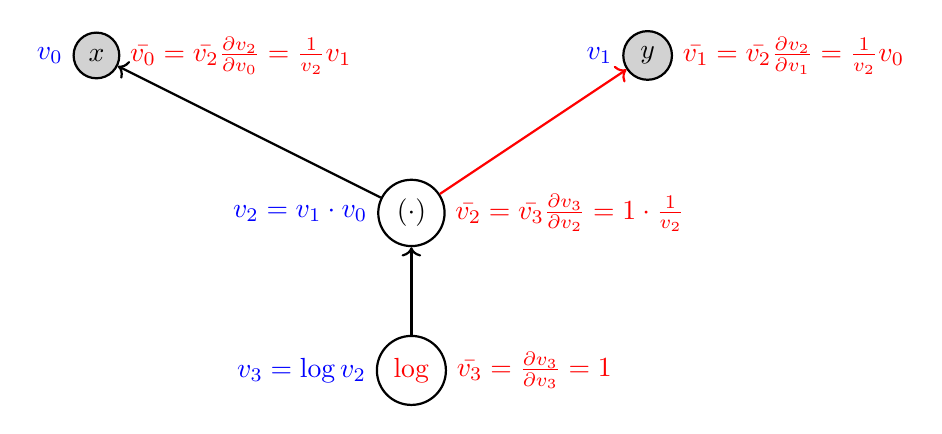
\begin{tikzpicture}
  [
    Round/.style={circle, draw=black!, fill=green!0, thick, minimum size=2mm},
    Red/.style={circle, draw=black!, fill=red!255, thick, minimum size=2mm},
    Yellow/.style={circle, draw=black!, fill=yellow!255, thick, minimum size=10mm},
    Gray/.style={circle, draw=black!, fill=gray!35, thick, minimum size=2mm}
  ]
  % Nodes
  \node[Gray, label=left:{\textcolor{blue}{$v_1$}},
    label=right:{\textcolor{red}{$\adj{v_1}=\adj{v_2}\pp{v_2}{v_1}=\frac{1}{v_2}v_0$}}] (v0) at(-1, 0) {$y$};
  \node[Gray, label=left:{\textcolor{blue}{$v_0$}},
    label=right:{\textcolor{red}{$\adj{v_0}=\adj{v_2}\pp{v_2}{v_0}=\frac{1}{v_2}v_1$}}] (v1) at(-8, 0) {$x$};
  \node[Round, label=left:{\textcolor{blue}{$v_2 = v_1 \cdot v_0$}},
    label=right:{\textcolor{red}{$\adj{v_2}=\adj{v_3}\pp{v_3}{v_2}=1\cdot \frac{1}{v_2}$}}] (v2) at(-4, -2) {$(\cdot)$};
  \node[Round, label=left:{\textcolor{blue}{$v_3 = \log{v_2}$}},
    label=right:{\textcolor{red}{$\adj{v_3}=\pp{v_3}{v_3}=1$}}] (v3) at(-4, -4) {$\mathcolor{red}{\log}$};
  % Lines
  \path [->, draw=red, thick] (v2) -- (v0);
  \path [->, draw, thick] (v2) -- (v1);
  \path [->, draw, thick] (v3) -- (v2);
\end{tikzpicture}
\end{frame}

\begin{frame}{Reverse Pass}
\vspace{-1mm}
$$z = \log(x\cdot y)$$
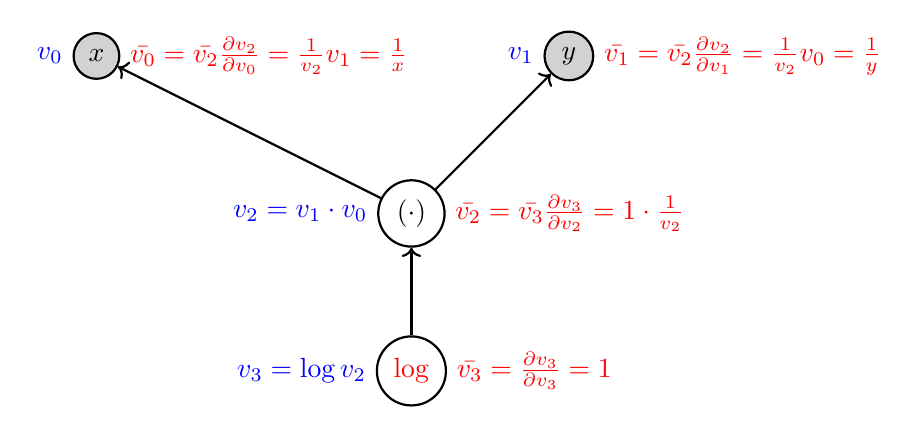
\begin{tikzpicture}
  [
    Round/.style={circle, draw=black!, fill=green!0, thick, minimum size=2mm},
    Red/.style={circle, draw=black!, fill=red!255, thick, minimum size=2mm},
    Yellow/.style={circle, draw=black!, fill=yellow!255, thick, minimum size=10mm},
    Gray/.style={circle, draw=black!, fill=gray!35, thick, minimum size=2mm}
  ]
  % Nodes
  \node[Gray, label=left:{\textcolor{blue}{$v_1$}},
    label=right:{\textcolor{red}{$\adj{v_1}=\adj{v_2}\pp{v_2}{v_1}=\frac{1}{v_2}v_0=\frac{1}{y}$}}] (v0) at(-2, 0) {$y$};
  \node[Gray, label=left:{\textcolor{blue}{$v_0$}},
    label=right:{\textcolor{red}{$\adj{v_0}=\adj{v_2}\pp{v_2}{v_0}=\frac{1}{v_2}v_1=\frac{1}{x}$}}] (v1) at(-8, 0) {$x$};
  \node[Round, label=left:{\textcolor{blue}{$v_2 = v_1 \cdot v_0$}},
    label=right:{\textcolor{red}{$\adj{v_2}=\adj{v_3}\pp{v_3}{v_2}=1\cdot \frac{1}{v_2}$}}] (v2) at(-4, -2) {$(\cdot)$};
  \node[Round, label=left:{\textcolor{blue}{$v_3 = \log{v_2}$}},
    label=right:{\textcolor{red}{$\adj{v_3}=\pp{v_3}{v_3}=1$}}] (v3) at(-4, -4) {$\mathcolor{red}{\log}$};
  % Lines
  \path [->, draw, thick] (v2) -- (v0);
  \path [->, draw, thick] (v2) -- (v1);
  \path [->, draw, thick] (v3) -- (v2);
\end{tikzpicture}
\note{We can think of AD operations as a function returning functions for the forward pass and the reverse pass}
\end{frame}

\end{comment}

\begin{frame}{What Do AD Libraries Care About?}
    \begin{itemize}
        \item Flexibility:
         \begin{itemize}
             \item Debugging, exceptions, conditional loops, matrix subset assignment
         \end{itemize}
         \item: Efficiency:
         \begin{itemize}
             \item Efficiently using a single CPU/GPU
         \end{itemize}
         \item Scaling
         \begin{itemize}
             \item Efficiently using clusters with multi-gpu/cpu nodes
         \end{itemize}
    \end{itemize}
\end{frame}
\note{..}

\begin{frame}{How do we keep track of our reverse pass?}
\begin{itemize}
  \item[] Source code transformation
    \begin{itemize}
        \item[-] Unroll all forward passes and reverse passes into one function
        \begin{itemize}
            \item[Good:] Fast
            \item[Bad:] Hard to implement, very restrictive
        \end{itemize}
    \end{itemize}

    \item[] Operator Overloading
    \begin{itemize}
        \item[-] Nodes in the expression graph are objects which store a forward and reverse pass function
        \begin{itemize}
          \item[Good:] Easier to implement, more flexible
          \item[Bad:] Less optimization opportunities
        \end{itemize}
    \end{itemize}
\end{itemize}
Newer AD packages use a combination of both
\end{frame}
\note{flexibility, performance, and developer time}

\begin{frame}{How do we keep track of our reverse pass?}
Static (Fast) vs. Dynamic (Flexible) graphs
\begin{itemize}
\item Known expression graph size at compile time? (Static)
\item Reassignment of variables (Dynamic easy, Static hard)
\item How much time do I have? (Dynamic)
\end{itemize}
\end{frame}
\note{..}

\begin{frame}{Operator Overloading Approach}
The operator overloading approach usually involves:
\begin{itemize}
    \item Runtime "tape" for tracking expressions
    \item Arena allocator for storing AD nodes
    \item Pair scalar type to hold the value and adjoint
\end{itemize}
%Allows conditional loops and reassignment of values in matrices\\
\end{frame}
\note{..}

\begin{comment}
\begin{frame}[fragile]{Cool graph math, how do we do this in a computer?}
\begin{minted}{C++}
auto foo_fwd(double x, double y);
\end{minted}
\end{frame}

\begin{frame}[fragile]{Cool graph math, how do we do this in a computer?}
\begin{minted}{C++}
auto foo_fwd(double x, double y);

template<ADType Ret, ADType T1, ADType T2>
auto foo_rev(Ret&& z, T1& x, T2& y) {
  adjoint(x) += adjoint(z) * compute_adj(x);
  adjoint(y) += adjoint(z) * compute_adj(y);
}
\end{minted}
\end{frame}

\begin{frame}[fragile]{Cool graph math, how do we do this in a computer?}
\begin{minted}{C++}
auto foo_fwd(double x, double y);
template<ADType Ret, ADType T1, ADType T2>
auto foo_rev(Ret&& z, T1&& x, T2&& y) {
  adjoint(x) += adjoint(z) * compute_adj(x);
  adjoint(y) += adjoint(z) * compute_adj(y);
}
template<ADType T1, ADType T2>
auto foo(T1&& x, T2&& y) {
  // Fwd pass
  auto fwd_ret = foo_fwd(value(x), value(y));
  // Setup reverse pass
  auto foo_rev = [](auto&& z, auto& x, auto& y) {
    return my_func_rev(z, x, y);
  };
  return tuple{foo_rev, fwd_ret, x, y};
}
\end{minted}
\end{frame}
\end{comment}

\begin{comment}
\begin{frame}[fragile]{Operator Overloading: Simple}
\begin{minted}{C++}
struct var_impl {
  double val_;
  double adj_;
  virtual void chain() {}
  var_impl(double val) : val_(val), adj_(0.0) {}
};
static std::vector<std::shared_ptr<var_impl>> tape;
struct var {
  std::shared_ptr<var_impl> vi_;
  var(std::shared_ptr<var_impl>& vi) : vi_(vi) {
    tape.push_back(vi);
  }
};
\end{minted}
\end{frame}

\begin{frame}[fragile]{Operator Overloading: Simple}
\begin{minted}{C++}
struct mul_vv final : public var_impl {
  var op1_;
  var op2_;
  mul_vv(double val, var op1, var op2) : var_impl(val), op1_(op1), op2_(op2) {}
  void chain() {
    op1_.adj() += op2_.val() * this->adjoint_;
    op2_.adj() += op1_.val() * this->adjoint_;
  }
};
operator*(var x, var y) {
  return var{
    std::make_shared<mul_vv>(
      x.val() * y.val(), x, y)};
}
\end{minted}
\note{The virtual function in var\_impl is a performance trick}
\end{frame}
\begin{frame}[fragile]{Operator Overloading: Simple}
\begin{minted}{C++}
void grad(var& v) {
  v.adj() = 1.0;
  for (auto&& x : tape | std::views::reverse) {
    x->chain();
  }
}
var x(2.0);
var y(4.0);
auto z = x;
while (value(z) < 10) {
  z += x * log(y) + log(x * y) * y;
}
grad(z);
\end{minted}
\href{https://github.com/SteveBronder/cppcon2025_autodiff/blob/main/code/benchmarks/shared_ptr.cpp}{\textcolor{blue}{Full Example}}
\note{At this point run the benchmark for shared}
\end{frame}


\begin{frame}{Issues}
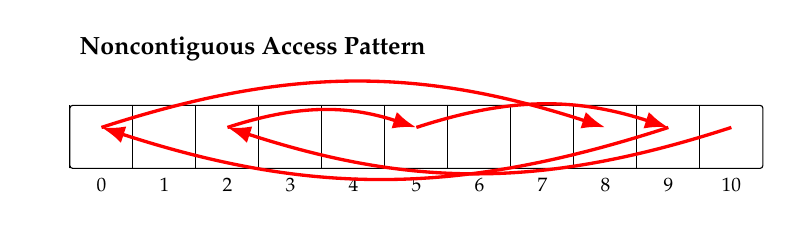
\begin{tikzpicture}[x=0.8cm,y=0.8cm,>=Latex,font=\small]
  % Config
  \def\N{11}                   % number of cells
  \def\cl{4}                   % cache-line size in cells
  \def\h{1.0}                  % cell height

  % Memory bar
  \draw[rounded corners=1pt] (0,0) rectangle (\N,\h);
  \foreach \i in {0,...,10} {
    \draw (\i,0) -- (\i,\h);
    \node[below] at (\i+0.5,0) {\scriptsize \i};
  }
  % Cache line boundaries

  % Access order (noncontiguous): change this list to your needs
  % Sequence: 1 → 9 → 3 → 12 → 5 → 14 → 2 → 11
  % markers

  % jumps (curved arrows)
  \draw[->,very thick,red,bend left=18]  (10.5,0.65) to (2.5,0.65);
  \draw[->,very thick,red,bend left=18]  (2.5,0.65) to (5.5,0.65);
  \draw[->,very thick,red,bend left=18]  (5.5,0.65) to (9.5,0.65);
  \draw[->,very thick,red,bend left=18]  (9.5,0.65) to (0.5,0.65);
  \draw[->,very thick,red,bend left=18]  (0.5,0.65) to (8.5,0.65);

  % legend
  \draw[very thick,black!45] (0,-0.55) -- (0.0,-0.55) node[left=8pt] {};
  \node[below left] at (0,-0.05) {};
  \node[above right,align=left] at (0,\h+0.55) {\bfseries Noncontiguous Access Pattern};
\end{tikzpicture}

\end{frame}
\begin{frame}{Issues}
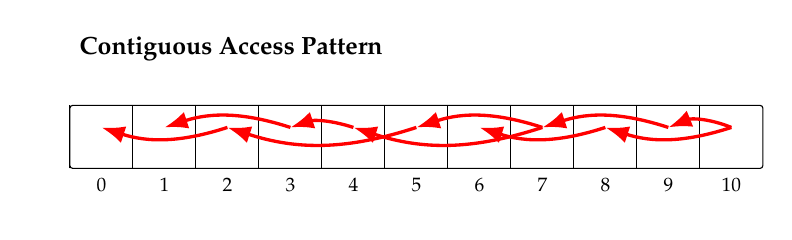
\begin{tikzpicture}[x=0.8cm,y=0.8cm,>=Latex,font=\small]
  % Config
  \def\N{11}                   % number of cells
  \def\cl{4}                   % cache-line size in cells
  \def\h{1.0}                  % cell height

  % Memory bar
  \draw[rounded corners=1pt] (0,0) rectangle (\N,\h);
  \foreach \i in {0,...,10} {
    \draw (\i,0) -- (\i,\h);
    \node[below] at (\i+0.5,0) {\scriptsize \i};
  }
  % Cache line boundaries

  % Access order (noncontiguous): change this list to your needs
  % Sequence: 1 → 9 → 3 → 12 → 5 → 14 → 2 → 11
  % markers

  % jumps (curved arrows)
  \draw[->,very thick,red,bend right=22] (10.5,0.65)  to (9.5,0.65);
  \draw[->,very thick,red,bend left=18]  (10.5,0.65) to (8.5,0.65);
  \draw[->,very thick,red,bend right=18]  (9.5,0.65) to (7.5,0.65);
  \draw[->,very thick,red,bend left=18]  (8.5,0.65) to (6.5,0.65);
  \draw[->,very thick,red,bend right=18]  (7.5,0.65) to (5.5,0.65);
  \draw[->,very thick,red,bend left=18]  (7.5,0.65) to (4.5,0.65);
  \draw[->,very thick,red,bend right=18]  (4.5,0.65) to (3.5,0.65);
  \draw[->,very thick,red,bend left=18]  (5.5,0.65) to (2.5,0.65);
  \draw[->,very thick,red,bend right=18]  (3.5,0.65) to (1.5,0.65);
  \draw[->,very thick,red,bend left=18]  (2.5,0.65) to (0.5,0.65);

  % legend
  \draw[very thick,black!45] (0,-0.55) -- (0.0,-0.55) node[left=8pt] {};
  \node[below left] at (0,-0.05) {};
  \node[above right,align=left] at (0,\h+0.55) {\bfseries Contiguous Access Pattern};
\end{tikzpicture}

\end{frame}
\end{comment}

\begin{comment}
\begin{frame}[fragile]{Operator Overloading Approach: Adolc}
\begin{minted}{C++}
enum class op_code {LOG_EXPR, ADD_EXPR, MUL_EXPR};
struct var_impl {
  double val;
  double adj;
}; // 12 bytes
struct var {
  var_impl* vi_;
}; // 8 bytes
\end{minted}
\end{frame}

\begin{frame}[fragile]{Operator Overloading Approach: Adolc}
\begin{minted}{C++}
struct ad_tape {
  struct expr_info {
    var_impl** out_;
    var_impl** in_;
    op_code chain_op;
  };
  std::vector<expr_info> tape_;
  inline void add_expr(var out, op_code expr_op,
    var in1, var in2) {
    tape_.push_back({out.vi_, {in1.vi_, in2.vi_}, expr_op});
    return out;
  }
};
static ad_tape g_tape{};
\end{minted}
\end{frame}

\begin{frame}[fragile]{Operator Overloading Approach: Adolc}
\begin{minted}{C++}
inline auto operator+(var x, var y) {
  return tape.add_expr(
    var(x.val() + y.val()), x, y, op_code::ADD_EXPR);
}
\end{minted}
\end{frame}

\begin{frame}[fragile]{Operator Overloading Approach}
\begin{minted}{C++}
void calc_grad(Tape& tape) {
  auto tape_val = tape.start();
  while (tape_val != tape.end()) {
    auto&& op = tape_val.get_op();
    switch (op.chain_op) {
      case LOG_EXPR:
       op.in(0).adj += op.out(0).adj * 1.0 / op.in(0).val;
      case MUL_EXPR:
       op.in(0).adj += op.out(0).adj * op.in(1).val;
       op.in(1).adj += op.out(0).adj * op.in(0).val;
    }
  }
}
\end{minted}
\end{frame}
\end{comment}

\begin{frame}[fragile]{Operator Overloading: Basic Type}
\begin{minted}{C++}
struct var_impl {
  double val;
  double adj;
  virtual void chain() {};
}; // 24 bytes
struct var {
  var_impl* vi_;
}; // 8 bytes
\end{minted}
\end{frame}
\note{var\_impl is our base type all expression nodes inherit from}

\begin{frame}[fragile]{Operator Overloading: Monotonic Buffer}
\begin{minted}{C++}
struct Tape {
std::monotonic_buffer_resource mbr{(1 << 16)};
std::polymorphic_allocator<std::byte> pa{&mbr};
std::vector<var_impl*> tape;
void clear() {
  tape.clear();
  mbr.release();
}
};
static Tape g_tape{};
template <typename T, typename Types>
auto new_node(Types&&... args) {
  auto* ret = g_tape.pa.template new_object<T>(args...);
  g_tape.tape.push_back(ret);
  return var{ret};
}
\end{minted}
\end{frame}
\note{..}

\begin{comment}
\begin{frame}[fragile]{Monotonic Buffer}
\begin{minted}{C++}
struct LogVari : var_impl {
  var_impl* in_;
  LogVari(var x) : in_(std::log(x.vi_->val)) {}
  virtual void chain() override {
    in_->adj += adj / in_->val;
  }
}; // 32 bytes
inline var log(var x) {
  return var(new_vari<LogVari>(x));
}
\end{minted}
\centering
\begin{CacheLine}
  % Color some blocks
  \CacheMarkBelow{0}{LogVari\{dbl, dbl, vptr, var_impl*\}}
  \CacheColor{0}{green!60}
  \CacheColor{1}{green!60}
  \CacheColor{2}{green!60}
  \CacheColor{3}{green!60}
  \CacheColor{4}{red!60}
  \CacheColor{5}{red!60}
  \CacheColor{6}{red!60}
  \CacheColor{7}{red!60}
\end{CacheLine}
\end{frame}
\end{comment}

\begin{frame}[fragile]{Operator Overloading: Expression Node}
\begin{minted}{C++}
struct mul_vv : public var_impl {
  var op1_;
  var op2_;
  void chain() {
    op1_.adj() += this->adjoint_ * op2_.val();
    op2_.adj += this->adjoint_ * op1_.val();
  }
}; // 40 bytes
var operator*(var op1, var op2) {
  return new_node<mul_vv>(op1.val() * op2.val(),
    op1, op2);
}
\end{minted}
\begin{comment}
\centering
\begin{CacheLine}
  % Color some blocks
  \CacheMarkBelow{0}{mul\_vv\{dbl, dbl, vptr, var\_impl*, var\_impl*\}}
  \CacheColor{0}{green!60}
  \CacheColor{1}{green!60}
  \CacheColor{2}{green!60}
  \CacheColor{3}{green!60}
  \CacheColor{4}{green!60}
  \CacheColor{5}{red!60}
  \CacheColor{6}{red!60}
  \CacheColor{7}{red!60}
\end{CacheLine}
\end{comment}
\end{frame}
\note{..}

\begin{frame}[fragile]{Operator Overloading: Reverse Pass}
\begin{minted}[escapeinside=||]{C++}
void grad(var& v) {
  v.adj = 1.0;
  for (auto&& x : tape | std::views::reverse) {
    x->chain();
  }
}
\end{minted}
\end{frame}
\note{..}

\begin{frame}[fragile]{Monotonic Buffer}
\begin{minted}[escapeinside=||]{C++}
void compute_grads(var x, var y) {
  var z = -10;
  while (z.val() < 20) {
    z += log(x * y);
  }
  grad(z);
}
// Later in program
for (int i = 0; i < 1e10; ++i) {
  var x = compute_x(...);
  var y = compute_y(...);
  compute_grads(x, y);
  do_something_with_grads(x.adj, y.adj);
  g_tape.clear();
}
\end{minted}
\end{frame}
\note{..}

\begin{frame}[fragile]{So Many Operator Classes}
\begin{minted}{C++}
struct mul_vv;
struct mul_vd;
struct mul_dv;
struct add_vv;
struct add_dv;
struct add_vd;
struct subtract_vv;
struct subtract_dv;
struct subtract_vd;
struct divide_vv;
struct divide_dv;
struct divide_vd;
\end{minted}
\end{frame}
\note{..}


\begin{frame}[fragile]{Reduce Boilerplate}
\begin{minted}[escapeinside=||]{C++}
template <Functor F>
struct callback_var_impl : public var_impl {
  F rev_functor_;
  template <std::floating_point S>
  explicit callback_var_impl(
    S&& value, F&& rev_functor)
    : var_impl(value),
      rev_functor_(rev_functor) {}
  void chain() final { rev_functor_(*this); }
}; // 24 + 8B * N
\end{minted}
\end{frame}
\note{..}

\begin{frame}[fragile]{Reduce Boilerplate}
\begin{minted}[escapeinside=||]{C++}
template <typename T1, typename T2>
requires any_var<T1, T2>
inline auto operator*(T1 op1, T2 op2) {
  return new_node<callback_var_impl>(
    value(op1) * value(op2),
    [op1, op2](auto&& ret) mutable {
      if constexpr (is_var_v<T1>) {
        adjoint(op1) += adjoint(ret) * value(op2);
      }
      if constexpr (is_var_v<T2>) {
        adjoint(op2) += adjoint(ret) * value(op1);
      }
    });
}
\end{minted}
\end{frame}
\note{..}

\begin{frame}{Poor Cache Use}
\begin{CacheLine}
  % Color some blocks
  \CacheMarkBelow{0}{var\_impl\{dbl, dbl, vptr\}}
  \CacheColor{0}{green!60}
  \CacheColor{1}{green!60}
  \CacheColor{2}{green!60}
  \CacheColor{3}{red!60}
  \CacheColor{4}{red!60}
  \CacheColor{5}{red!60}
  \CacheColor{6}{red!60}
  \CacheColor{7}{red!60}
\end{CacheLine}
\begin{CacheLine}
  % Color some blocks
  \CacheMarkBelow{0}{unary\_var\{dbl, dbl, vptr, var\_impl*\}}
  \CacheColor{0}{green!60}
  \CacheColor{1}{green!60}
  \CacheColor{2}{green!60}
  \CacheColor{3}{green!60}
  \CacheColor{4}{red!60}
  \CacheColor{5}{red!60}
  \CacheColor{6}{red!60}
  \CacheColor{7}{red!60}
\end{CacheLine}
\begin{CacheLine}
  % Color some blocks
  \CacheMarkBelow{0}{binary\_var\{dbl, dbl, vptr, var\_impl*, var\_impl*\}}
  \CacheColor{0}{green!60}
  \CacheColor{1}{green!60}
  \CacheColor{2}{green!60}
  \CacheColor{3}{green!60}
  \CacheColor{4}{green!60}
  \CacheColor{5}{red!60}
  \CacheColor{6}{red!60}
  \CacheColor{7}{red!60}
\end{CacheLine}
\end{frame}
\note{..}

\begin{frame}[fragile]{Source Code Transform Ex:}
\begin{minted}[escapeinside=||]{C++}
double z = log(x * y);
\end{minted}
Break it down
\begin{minted}[escapeinside=||]{C++}
double v0 = x;
double v1 = y;
double v2 = x * y;
double v3 = log(v2)
double bar_v3 = 1;
double bar_v2 = bar_v3 * 1/v2;
double bar_v1 = bar_v2 * v0;
double bar_v0 = bar_v2 * v1;
\end{minted}
\end{frame}
\note{..}

\begin{frame}[fragile]{Source Code Transform Ex:}
Code like the following very hard / impossible in source code transform
\begin{minted}[escapeinside=||]{C++}
while(error < tolerance) {
  // ...
}
\end{minted}
\end{frame}
\note{..}

\begin{frame}[fragile]{Source Code Transform Ex:}
\begin{minted}[escapeinside=||]{C++}
struct var {
    double values_;
    double adjoints_;
    var(double x) : values_(x), adjoints_(0) {}
};

\end{minted}
\end{frame}
\note{..}

\begin{frame}[fragile]{Source Code Transform Ex:}
\begin{minted}[escapeinside=||]{C++}
template <typename F, typename... Exprs>
struct expr {
   var ret_;
   std::tuple<deduce_ownership_t<Exprs>...> exprs_;
   std::decay_t<F> f_;
   template <typename FF, typename... Args>
   expr(double x, FF&& f, Args&&... args) :
     ret_(x), f_(std::forward<F>(f)),
     exprs_(std::forward<Args>(args)...) {}
};
\end{minted}
\end{frame}
\note{..}

\begin{frame}[fragile]{Source Code Transform Ex:}
\begin{minted}[escapeinside=||]{C++}
template <typename T1, typename T2>
requires any_var_or_expr<T1, T2>
inline auto operator*(T1&& lhs, T2&& rhs) {
  return make_expr(value(lhs) * value(rhs),
  [](auto&& ret, auto&& lhs, auto&& rhs) {
    if constexpr (!std::is_arithmetic_v<T1>) {
      adjoint(lhs) += adjoint(ret) * value(rhs);
    }
    if constexpr (!std::is_arithmetic_v<T2>) {
      adjoint(rhs) += adjoint(ret) * value(lhs);
    }
  }, std::forward<T1>(lhs), std::forward<T2>(rhs));
}
\end{minted}
\end{frame}
\note{..}

\begin{frame}[fragile]{Source Code Transform Ex:}
\begin{minted}[escapeinside=||]{C++}
auto z = x |{\mathcolor{red}{*}}| |{\mathcolor{cyan}{log}}|(y) |{\mathcolor{yellow}{+}}| |{\mathcolor{orange}{log}}|(x |{\mathcolor{lime}{*}}| y) |{\mathcolor{magenta}{*}}| y;
|{\mathcolor{yellow}{expr<Lambda<Plus>}}|,
  |{\mathcolor{red}{expr<Lambda<Mult>}}|, var, |{\mathcolor{cyan}{expr<Lambda<Log>}}|, var>>,
  |{\mathcolor{magenta}{expr<Lambda<Mult>}}|,
   |{\mathcolor{orange}{expr<Lambda<Log>}}|, |{\mathcolor{lime}{expr<Lambda<Mult>}}|, var, var>>,
   var>>
\end{minted}
\end{frame}
\note{..}

\begin{frame}[fragile]{Source Code Transform Ex:}
\begin{minted}{C++}
template <typename Expr>
inline void grad(Expr&& z) {
  adjoint(z) = 1.0;
  auto nodes = collect_bfs(z);
  eval_breadthwise(nodes);
}
\end{minted}
\centerline{\href{https://godbolt.org/z/veexMT5vz}{\textcolor{blue}{Example Godbolt}}}
\end{frame}
\note{..}

\begin{comment}
  auto z = + (* x (log y)) (* (log (* x y)) y)
\end{comment}

\begin{frame}{Comparison}
\begin{table}
  \centering % Centers the table on the page
  \caption{$f(x, y) = x\log(y) + \log(xy) y$;} % Table caption
  \label{tab:firsttable} % Label for referencing
  \begin{tabular}{|l|r|c|} % Three columns: left, center, right, with vertical lines
    \hline % Top horizontal line
    Method & CPU Time & \% Improvement \\ % First row (headers)
    \hline % Line after headers
    Shared Ptr & 508ns & 1.0 \\
    MonoBuff   & 121ns & 3.9x \\
    Lambda     & 112ns & 4.2x \\
    Source Code Transform        &  26.5ns & 19x \\
    Baseline & 2.82ns & 180x\\
    \hline % Bottom horizontal line
  \end{tabular}
\end{table}
\end{frame}
\note{..}

\begin{frame}[fragile]{Operator Overloading Approach: Matrices}
\begin{minted}{C++}
Matrix<var> B(M, M);
Matrix<var> X(M, M);
Matrix<var> Z = X * B.transpose();
\end{minted}
\end{frame}
\note{..}

\begin{frame}[fragile]{Operator Overloading Approach: Matrices}
\begin{minted}{C++}
template <typename MatrixType>
struct arena_matrix :
  public Eigen::Map<MatrixType> {
  using Base = Eigen::Map<MatrixType>
  template <typename T>
  arena_matrix(T&& mat) :
   Base(copy_to_arena(mat.data(), mat.size()),
     mat.rows(), mat.cols()) {}
};
\end{minted}
\end{frame}
\note{..}

\begin{frame}[fragile]{Operator Overloading Approach: Matrices}
\begin{minted}{C++}
// Array of Structs
struct Matrix<var> {
  var* data_;
};
// Struct of Arrays
struct var_impl<Matrix<double>> {
  arena_matrix<double> value_;
  arena_matrix<double> adjoint_;
  virtual void chain() {}
};
\end{minted}
\vspace{-8mm}
\end{frame}
\note{..}

\begin{frame}[fragile]{Operator Overloading Approach: Matrices}
\begin{minted}{C++}
// Array of Structs
struct Matrix<var> {
  var* data_;
};
\end{minted}
\begin{itemize}
    \item Array of Structs:
    \begin{itemize}
        \item Simple, most algorithms Just Work\texttrademark
        \item Adds a lot to expression graph
        \item turns off SIMD
    \end{itemize}
\end{itemize}
\end{frame}
\note{..}

\begin{frame}[fragile]{Operator Overloading Approach: Matrices}
\begin{minted}{C++}
// Struct of Arrays
struct var_impl<Matrix<double>> {
  arena_matrix<double> value_;
  arena_matrix<double> adjoint_;
  virtual void chain() {}
};
\end{minted}
\begin{itemize}
    \item Struct of Arrays:
    \begin{itemize}
        \item Hard, everything written out manually
        \item Collapses matrix expressions in tree
        \item SIMD can be used on values and adjoints
    \end{itemize}
\end{itemize}
\end{frame}
\note{..}

\begin{comment}
\begin{frame}[fragile]{Operator Overloading Approach: Matrices}
\begin{CacheLine}
  % Color some blocks
  \CacheMarkBelow{0}{var\_impl<Matrix>\{dbl*, dbl*, vptr\}}
  \CacheColor{0}{green!60}
  \CacheColor{1}{green!60}
  \CacheColor{2}{green!60}
  \CacheMarkAbove{3}{var\_impl<Matrix>\{dbl*, dbl*, vptr\}}
  \CacheColor{3}{green!60}
  \CacheColor{4}{green!60}
  \CacheColor{5}{green!60}
  \CacheColor{6}{red!60}
  \CacheColor{7}{red!60}
\end{CacheLine}
\end{frame}
\end{comment}
\begin{frame}[fragile]{Matrix Multiplication Example}
\begin{minted}{C++}
template <typename T1, typename T2>
requires any_var_matrix<T1, T2>
inline auto operator*(T1&& op1, T2&& op2) {
  return lambda_var(value(op1) * value(op2),
    [op1, op2](auto&& ret) mutable {
      if constexpr (is_var_matrix_v<T1>) {
        adjoint(op1) += adjoint(ret) * value(op2).transpose();
      }
      if constexpr (is_var_matrix_v<T2>) {
        adjoint(op2) += value(op1) * adjoint(ret);
      }
    });
}
\end{minted}
\end{frame}
\note{..}

\begin{frame}[fragile]{Operator Overloading Approach: Matrices}
\centering
\begin{CacheLine}
  % Color some blocks
  \CacheMarkBelow{0}{mat\_mul\_vv\{dbl*, dbl*, long int, long int, vptr, lambda[var<Mat>, var<Mat>]\}}
  \CacheColor{0}{green!60}
  \CacheColor{1}{green!60}
  \CacheColor{2}{green!60}
  \CacheColor{3}{green!60}
  \CacheColor{4}{green!60}
  \CacheColor{5}{green!60}
  \CacheColor{6}{green!60}
  \CacheColor{7}{green!60}
\end{CacheLine}
\end{frame}
\note{..}


\begin{frame}{Matrix Multiplication Benchmark}
\begin{figure}
\centerline{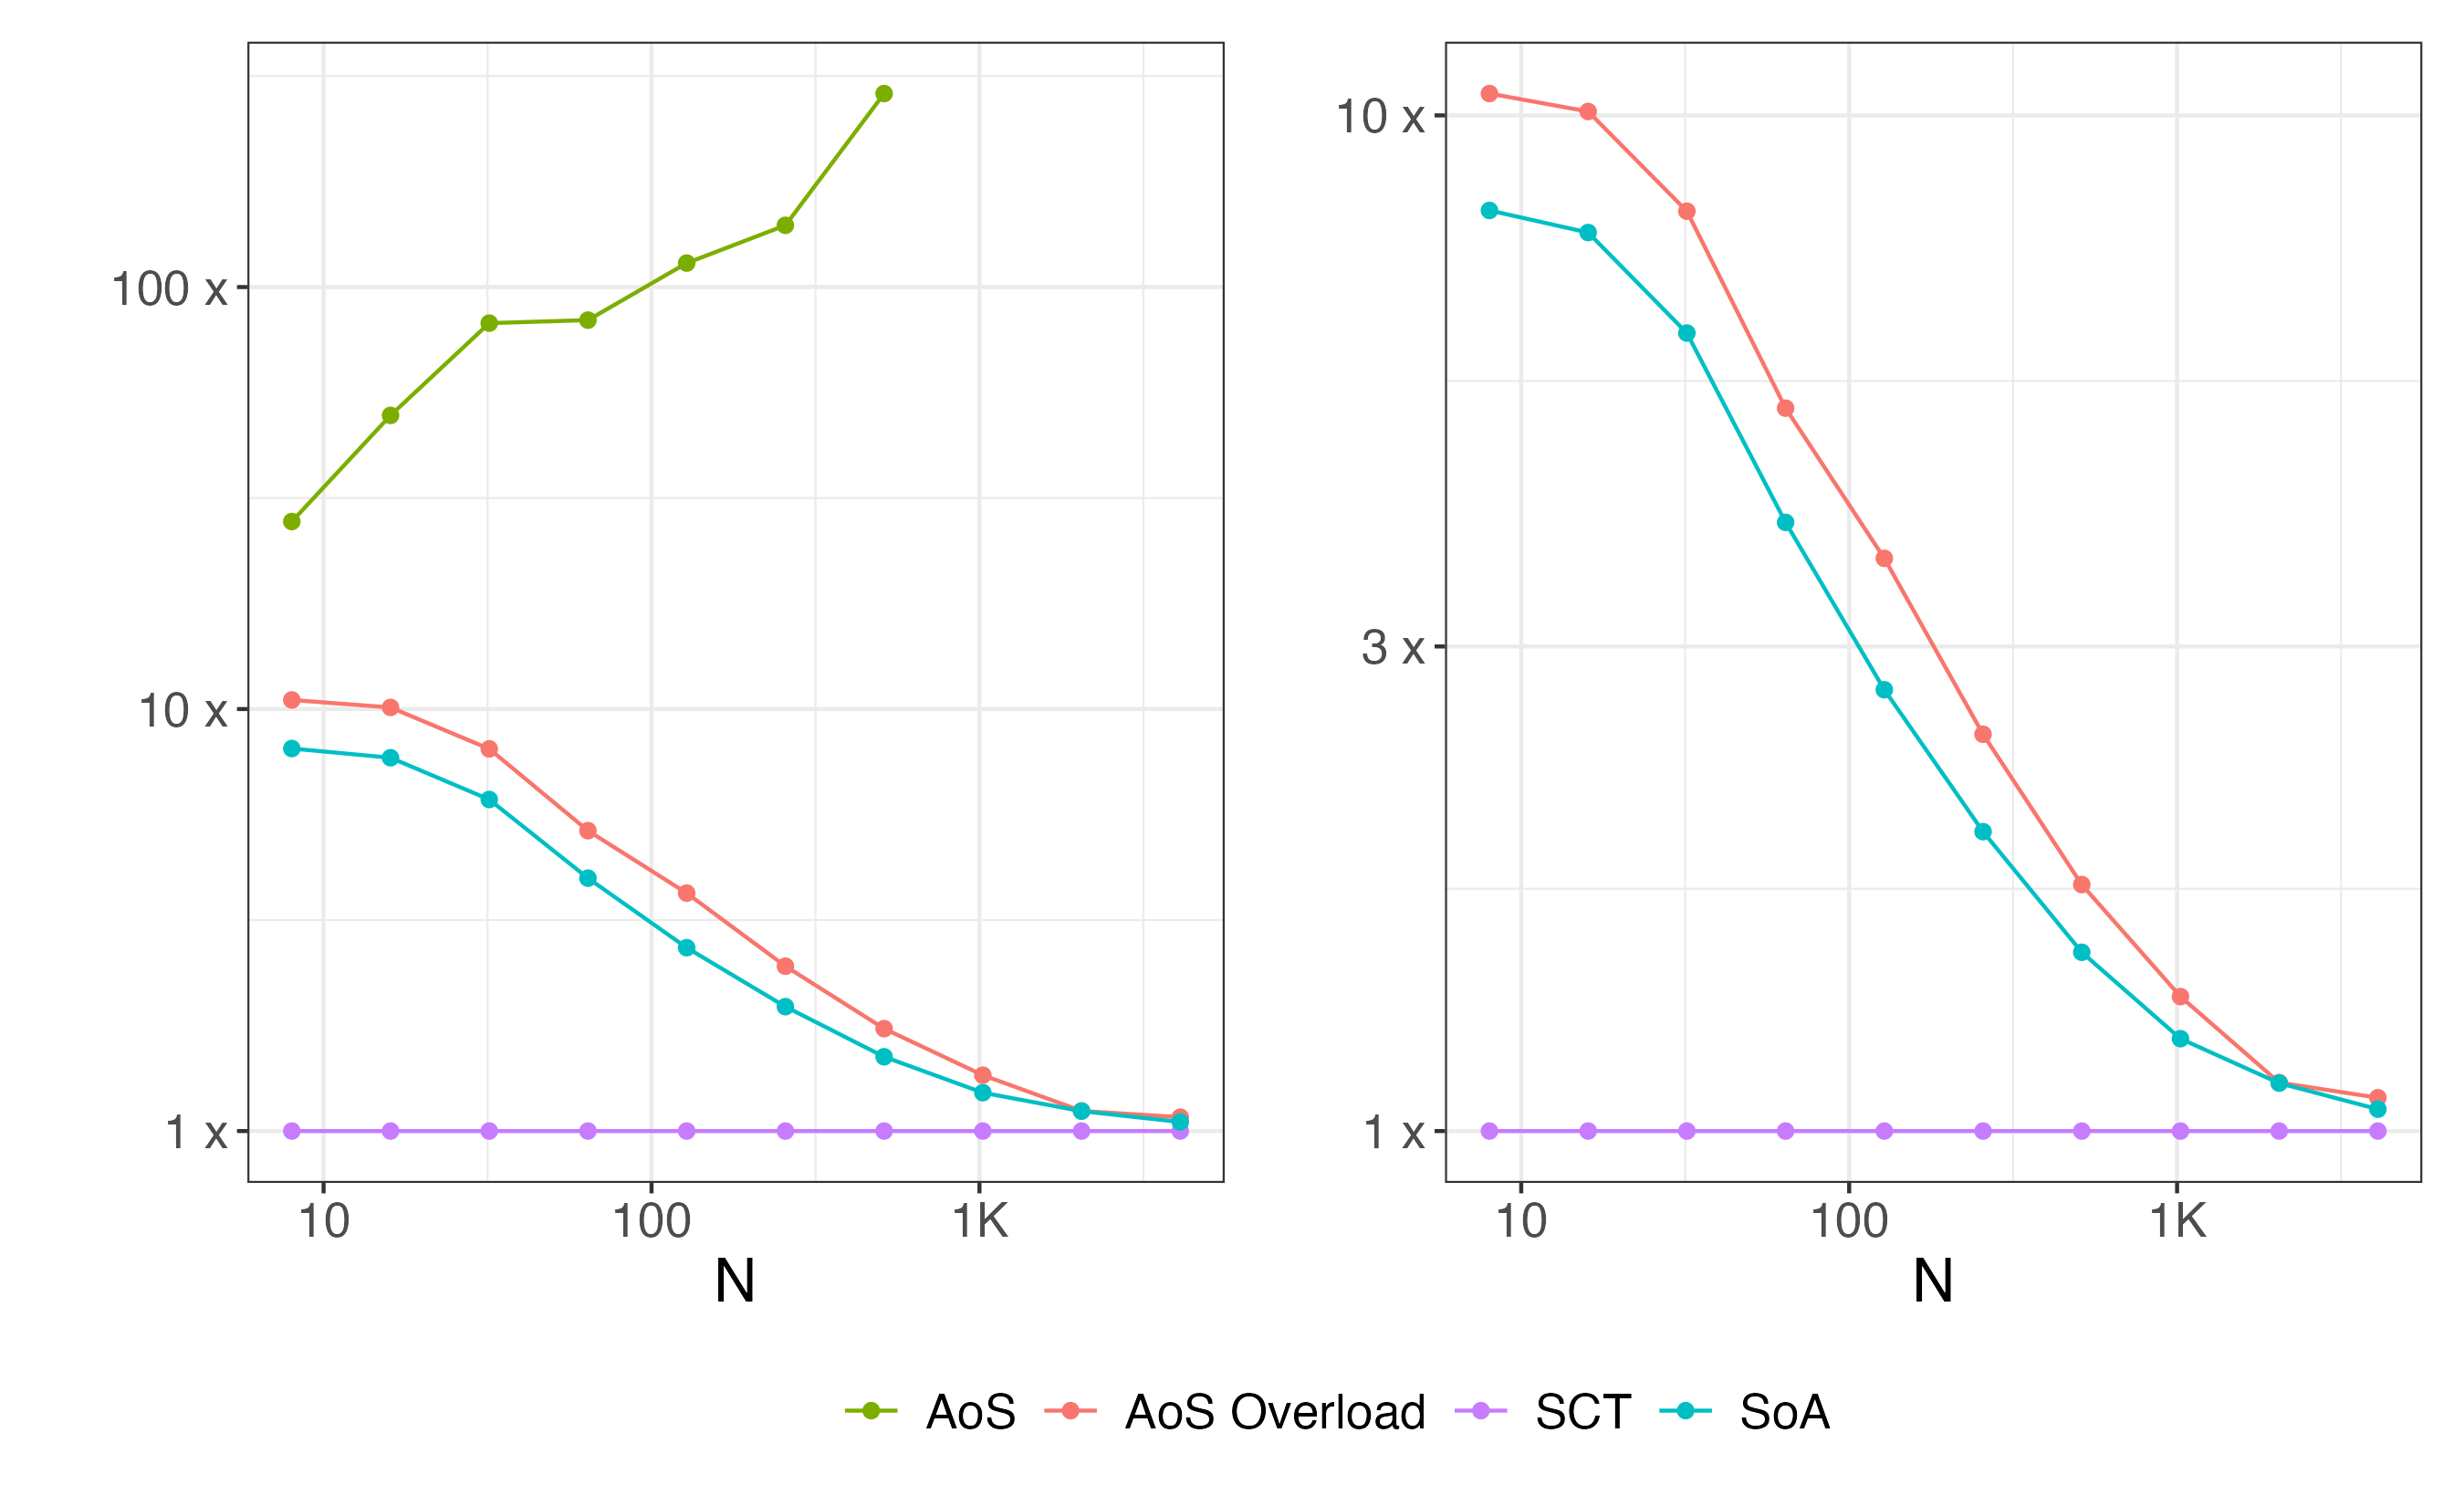
\includegraphics[scale=.5]{img/matmul_bench.png}}
\label{fig-matmul}
\end{figure}
\end{frame}
\note{..}

\begin{frame}[fragile]{Subset Assignment}
\vspace{-1mm}
\begin{minted}{C++}
var<Vector<double>> y{{0, 1, 2, 3}};
var<Vector<double>> x{{0, 1, 2, 3}};
var prod = y.dot(x);
x.slice(1, 3) = x.head(3);
auto z = prod + sum(x);
\end{minted}
\pause
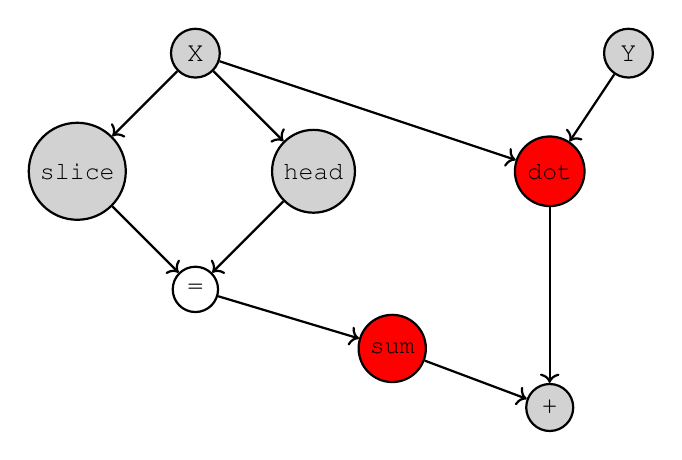
\begin{tikzpicture}
  [
    Round/.style={circle, draw=black!, fill=green!0, thick, minimum size=2mm},
    Red/.style={circle, draw=black!, fill=red!255, thick, minimum size=2mm},
    Yellow/.style={circle, draw=black!, fill=yellow!255, thick, minimum size=10mm},
    Gray/.style={circle, draw=black!, fill=gray!35, thick, minimum size=2mm}
  ]
  % Nodes (x, y)
  \node[Gray] (v0) at(-2.5, 0) {\texttt{X}};
  \node[Gray] (v1) at(3, 0) {\texttt{Y}};
  \small
  \node[Gray] (v2) at(-1, -1.5) {\texttt{head}};
  \node[Gray] (v3) at(-4, -1.5) {\texttt{slice}};
  \normalsize
  \node[Round] (v4) at(-2.5, -3) {\texttt{=}};
  \small
  \node[Red] (v5) at(2, -1.5) {\texttt{dot}};
  \node[Red] (v6) at(0, -3.75) {\texttt{sum}};
  \normalsize
  \node[Gray] (v7) at(2, -4.5) {\texttt{+}};

  % Lines
  % X.head()
  \path [<-, draw, thick] (v2) -- (v0);
  % X.slice()
  \path [<-, draw, thick] (v3) -- (v0);
  % = x.head()
  \path [<-, draw, thick] (v4) -- (v2);
  % x.slice() =
  \path [<-, draw, thick] (v4) -- (v3);
  % dot(x, _)
  \path [<-, draw, thick] (v5) -- (v0);
  % dot(_, y)
  \path [<-, draw, thick] (v5) -- (v1);
  % = -> sum(x)
  \path [<-, draw, thick] (v6) -- (v4);
  % sum(x) + _
  \path [<-, draw, thick] (v7) -- (v5);
  % _ + dot
  \path [<-, draw, thick] (v7) -- (v6);

\end{tikzpicture}
\end{frame}
\note{..}

\begin{frame}[fragile]{Subset Assignment}
\vspace{-1mm}
\begin{minted}{C++}
var<Vector<double>> y{{0, 1, 2, 3}};
var<Vector<double>> x{{0, 1, 2, 3}};
var prod = y.dot(x);
x.slice(1, 3) = x.head(3);
auto z = prod + sum(x);
\end{minted}
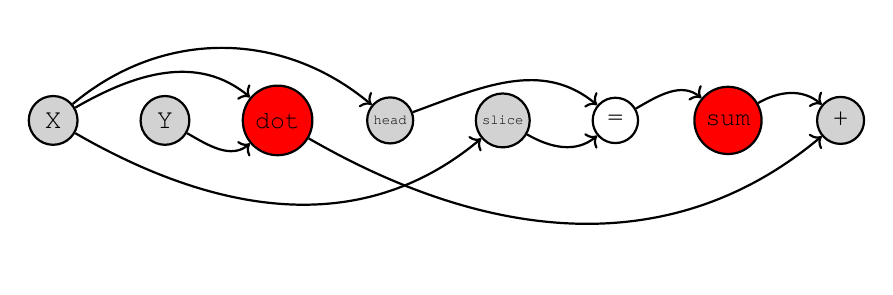
\begin{tikzpicture}
  [
    Round/.style={circle, draw=black!, fill=green!0, thick, minimum size=2mm},
    Red/.style={circle, draw=black!, fill=red!255, thick, minimum size=2mm},
    Yellow/.style={circle, draw=black!, fill=yellow!255, thick, minimum size=10mm},
    Gray/.style={circle, draw=black!, fill=gray!35, thick, minimum size=2mm}
  ]
  % Nodes (x, y)
  \node[Gray] (v0) at(0, 0) {\texttt{X}};
  \node[Gray] (v1) at(1.42, 0) {\texttt{Y}};
  \tiny
  \node[Gray] (v2) at(4.28, 0) {\texttt{head}};
  \node[Gray] (v3) at(5.71,  0) {\texttt{slice}};
  \normalsize
  \node[Round] (v4) at(7.14, 0) {\texttt{=}};
  \small
  \node[Red] (v5) at(2.85, 0) {\texttt{dot}};
  \node[Red] (v6) at(8.57, 0) {\texttt{sum}};
  \normalsize
  \node[Gray] (v7) at(10, 0) {\texttt{+}};

  % Lines
  % X.head()
  \path [<-, draw, thick] (v2) to[out=140,in=40] (v0);
  % X.slice()
  \path [<-, draw, thick] (v3) to[out=-140,in=-30] (v0);
  % = x.head()
  \path [<-, draw, thick] (v4) to[out=140,in=20] (v2);
  % x.slice() =
  \path [<-, draw, thick] (v4) to[out=-140,in=-30] (v3);
  % dot(x, _)
  \path [<-, draw, thick] (v5) to[out=140,in=30] (v0);
  % dot(_, y)
  \path [<-, draw, thick] (v5) to[out=-140,in=-30] (v1);
  % = -> sum(x)
  \path [<-, draw, thick] (v6) to[out=140,in=30] (v4);
  % sum(x) + _
  \path [<-, draw, thick] (v7) to[out=-140,in=-30] (v5);
  % _ + dot
  \path [<-, draw, thick] (v7) to[out=140,in=30] (v6);

\end{tikzpicture}
\end{frame}
\note{..}

\begin{frame}[fragile]{Subset Assignment Becomes Very Hard}
\begin{minted}{C++}
var<Vector<double>> x{{0, 1, 2, 3}};
x.slice(1, 3) = x.head(3);
\end{minted}

\begin{table}
  \centering % Centers the table on the page
  \label{tab:aliasing} % Label for referencing
  \begin{tabular}{|l|r|c|} % Three columns: left, center, right, with vertical lines
    \hline % Top horizontal line
    Iter & X \\ % First row (headers)
    \hline % Line after headers
    0 & \{0, 0, 2, 3\} \\
    1 & \{0, 0, 0, 3\} \\
    2 & \{0, 0, 0, 0\} \\
    \hline % Bottom horizontal line
  \end{tabular}
\end{table}
\end{frame}
\note{..}

\begin{frame}[fragile]{Subset Assignment Becomes Very Hard}
\begin{minted}{C++}
tempalte <typename T>
struct var {
template <typename S>
require AssignableExpression<T, S>
inline var<T>& operator=(const var<S>& other) {
  arena_matrix<T> prev_val(vi_->val_.rows(), vi_->val_.cols());
  prev_val.deep_copy(vi_->val_);
  vi_->val_.deep_copy(other.val());
  g_tape.callback(
  [this_vi = this->vi_, other_vi = other.vi_, prev_val]() mutable {
    this_vi->val_.deep_copy(prev_val);
    prev_val.deep_copy(this_vi->adj_);
    this_vi->adj_.setZero();
    other_vi->adj_ += prev_val;
  });
  return *this;
}
}
\end{minted}
\end{frame}
\note{..}

\begin{frame}{Thanks!}
Repository for benchmarks and slides
\begin{figure}
\centerline{
\includegraphics[scale=.1]{img/qr-code.png}}
\label{fig-qr-code}
\end{figure}
\end{frame}
\note{..}

\begin{comment}
\begin{frame}{Embarassingly Parallel Not Possible}
  But reduce sum style very easy
\end{frame}

\begin{frame}[fragile]{Scaling Up: CPU}
  \begin{itemize}
    \item Within a node, parallelism is easy
    \pause
    \item Parallel + static globals????
    \pause
    \item Yes, \pause sometimes
  \end{itemize}
\note{We have a ton of static globals, how are supposed to run this stuff in parallel? thread\_local duh! Going to hand wave away observer model for now }
\end{frame}


\begin{frame}[fragile]{Scaling Up: CPU}
\begin{minted}{C++}
struct ad_tape {
  struct ad_tape_instance {
    monotonic_buffer_resource mbr{1<<16};
    polymorphic_allocator<std::byte> pa{&mbr};
    std::vector<var_impl*> tape;
    void clear();
  };
  static thread_local ad_tape_instance* instance_;
  static void init();
};
thread_local ad_tape_instance* ad_tape::instance_;
\end{minted}
\end{frame}

\begin{frame}[fragile]{Scaling Up: CPU}
\begin{minted}{C++}
struct ad_tape_obs final : tbb::task_scheduler_observer {
  using tape_ptr = std::unique_ptr<ad_tape>;
  std::unordered_map<std::thread::id, tape_ptr> by_thread_;
  std::mutex m_;
  void on_scheduler_entry(bool /*worker*/);
  void on_scheduler_exit(bool /*worker*/);
};
\end{minted}
\end{frame}

\begin{frame}[fragile]{Scaling Up: CPU}
\begin{minted}{C++}
void on_scheduler_entry(bool /*worker*/) override {
  std::scoped_lock lk(m_);
  auto id = std::this_thread::get_id();
  auto& p = by_thread_[id];
  if (!p) p = std::make_unique<ad_tape>();
  tls_tape = p.get();
}
\end{minted}
\end{frame}

\begin{frame}[fragile]{Scaling Up: CPU}
\begin{minted}{C++}
void on_scheduler_exit(bool /*worker*/) override {
  std::scoped_lock lk(m_);
  by_thread_.erase(std::this_thread::get_id());
}
\end{minted}
\end{frame}
\end{comment}



\end{document}
